\chapter{Additional Data and Figures}
\label{appb:data}

\section{Full MP2 Reference Energies}

Here we include the MP2 correlation energy OVOS plots for the smaller 6--31G basis set.

\begin{figure}[H]
    \centering
    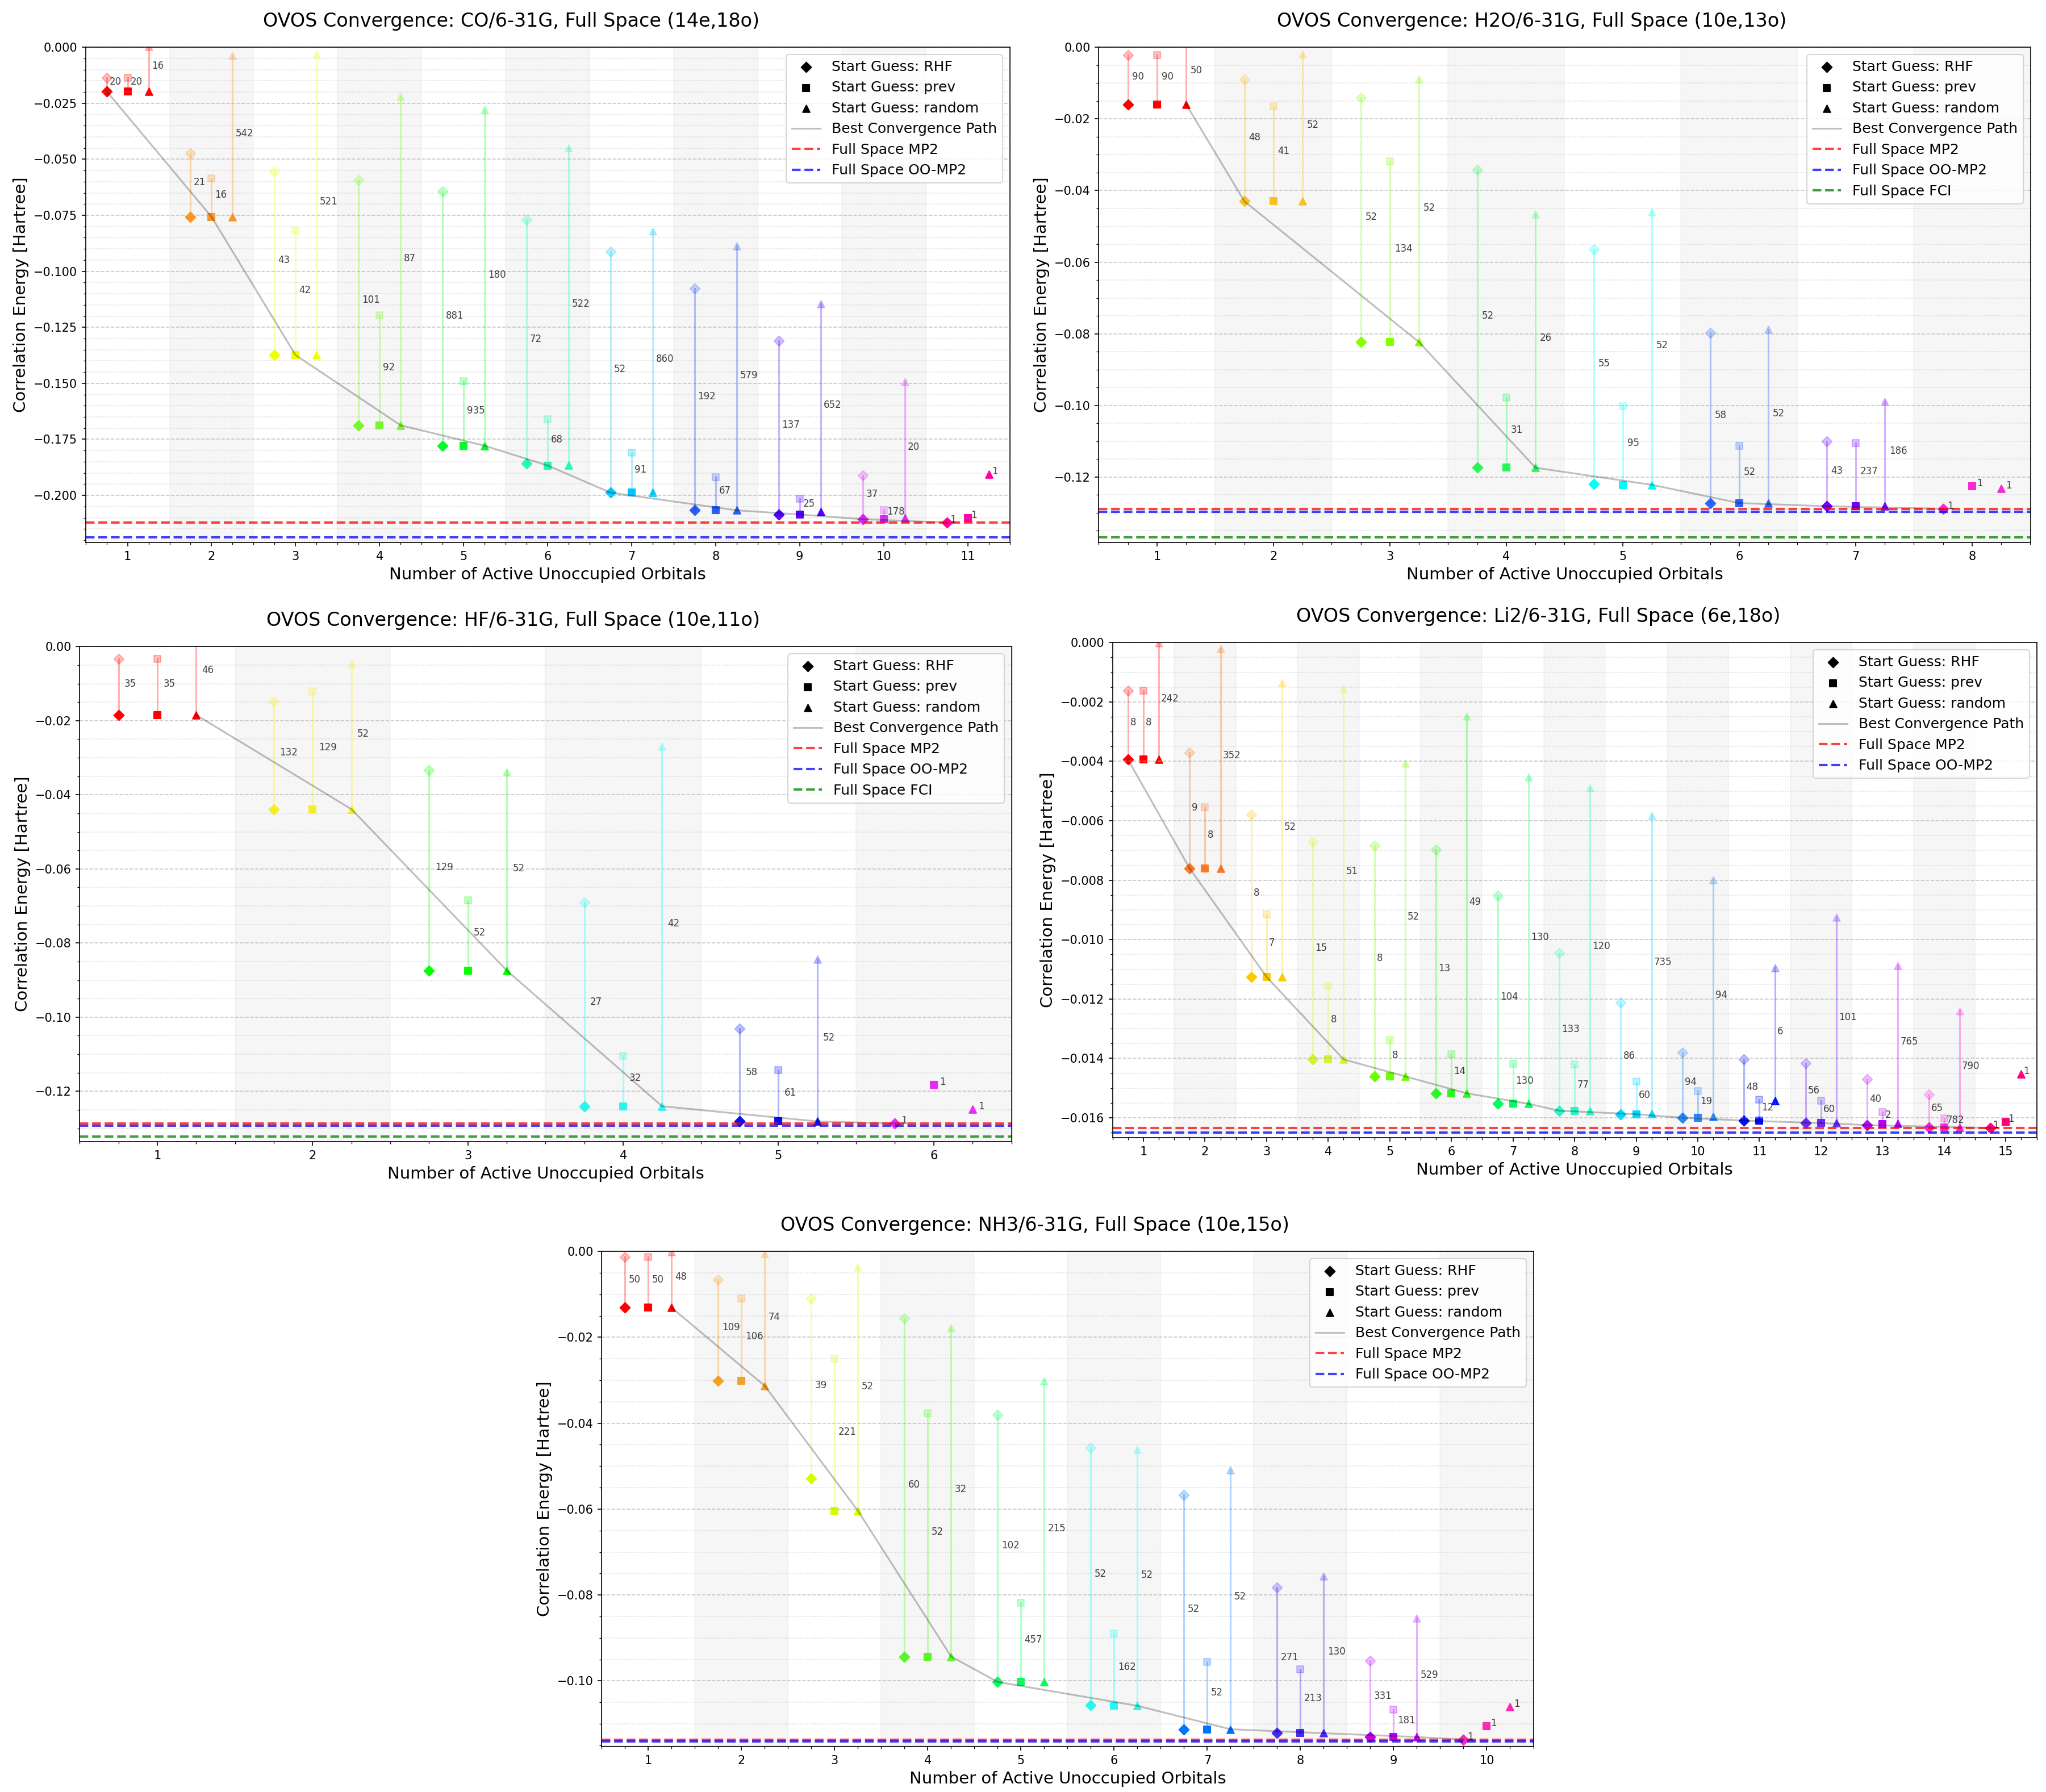
\includegraphics[width=0.9\textwidth]{figures/Ekstra/OVOS_6-31G.png}
    \caption{Convergence of the MP2 correlation energy for CO, H$_2$, HF, NH$_3$, and Li$_2$ in 6--31G basis, at each number of active unoccupied orbitals $N'_{act.unocc}$. The OVOS algorithm takes RHF (diamond), previous (square), and random (triangle) as start guesses. Dashed red line marks the MP2 correlation energy at full space, PySCF reference. Dashed lines: full-space MP2 (red), OO-MP2 (blue), FCI (green) references. A gray line is drawn to connect the best points of the start guesses. A line for each OVOS connects initial and final correlation energies, at which the number of iterations to convergence is annotated.}
    \label{fig:appb_MP2_6-31G_ovos}
\end{figure}







\section{Convergence Plots for All Systems}

Here we include the convergence plots for all systems, which show the energy recovery as a function of iteration number for each (molecule, basis) combination. These plots provide insight into the convergence behaviour of the OVOS algorithm across different systems and basis sets.

\begin{figure}[H]
    \centering
    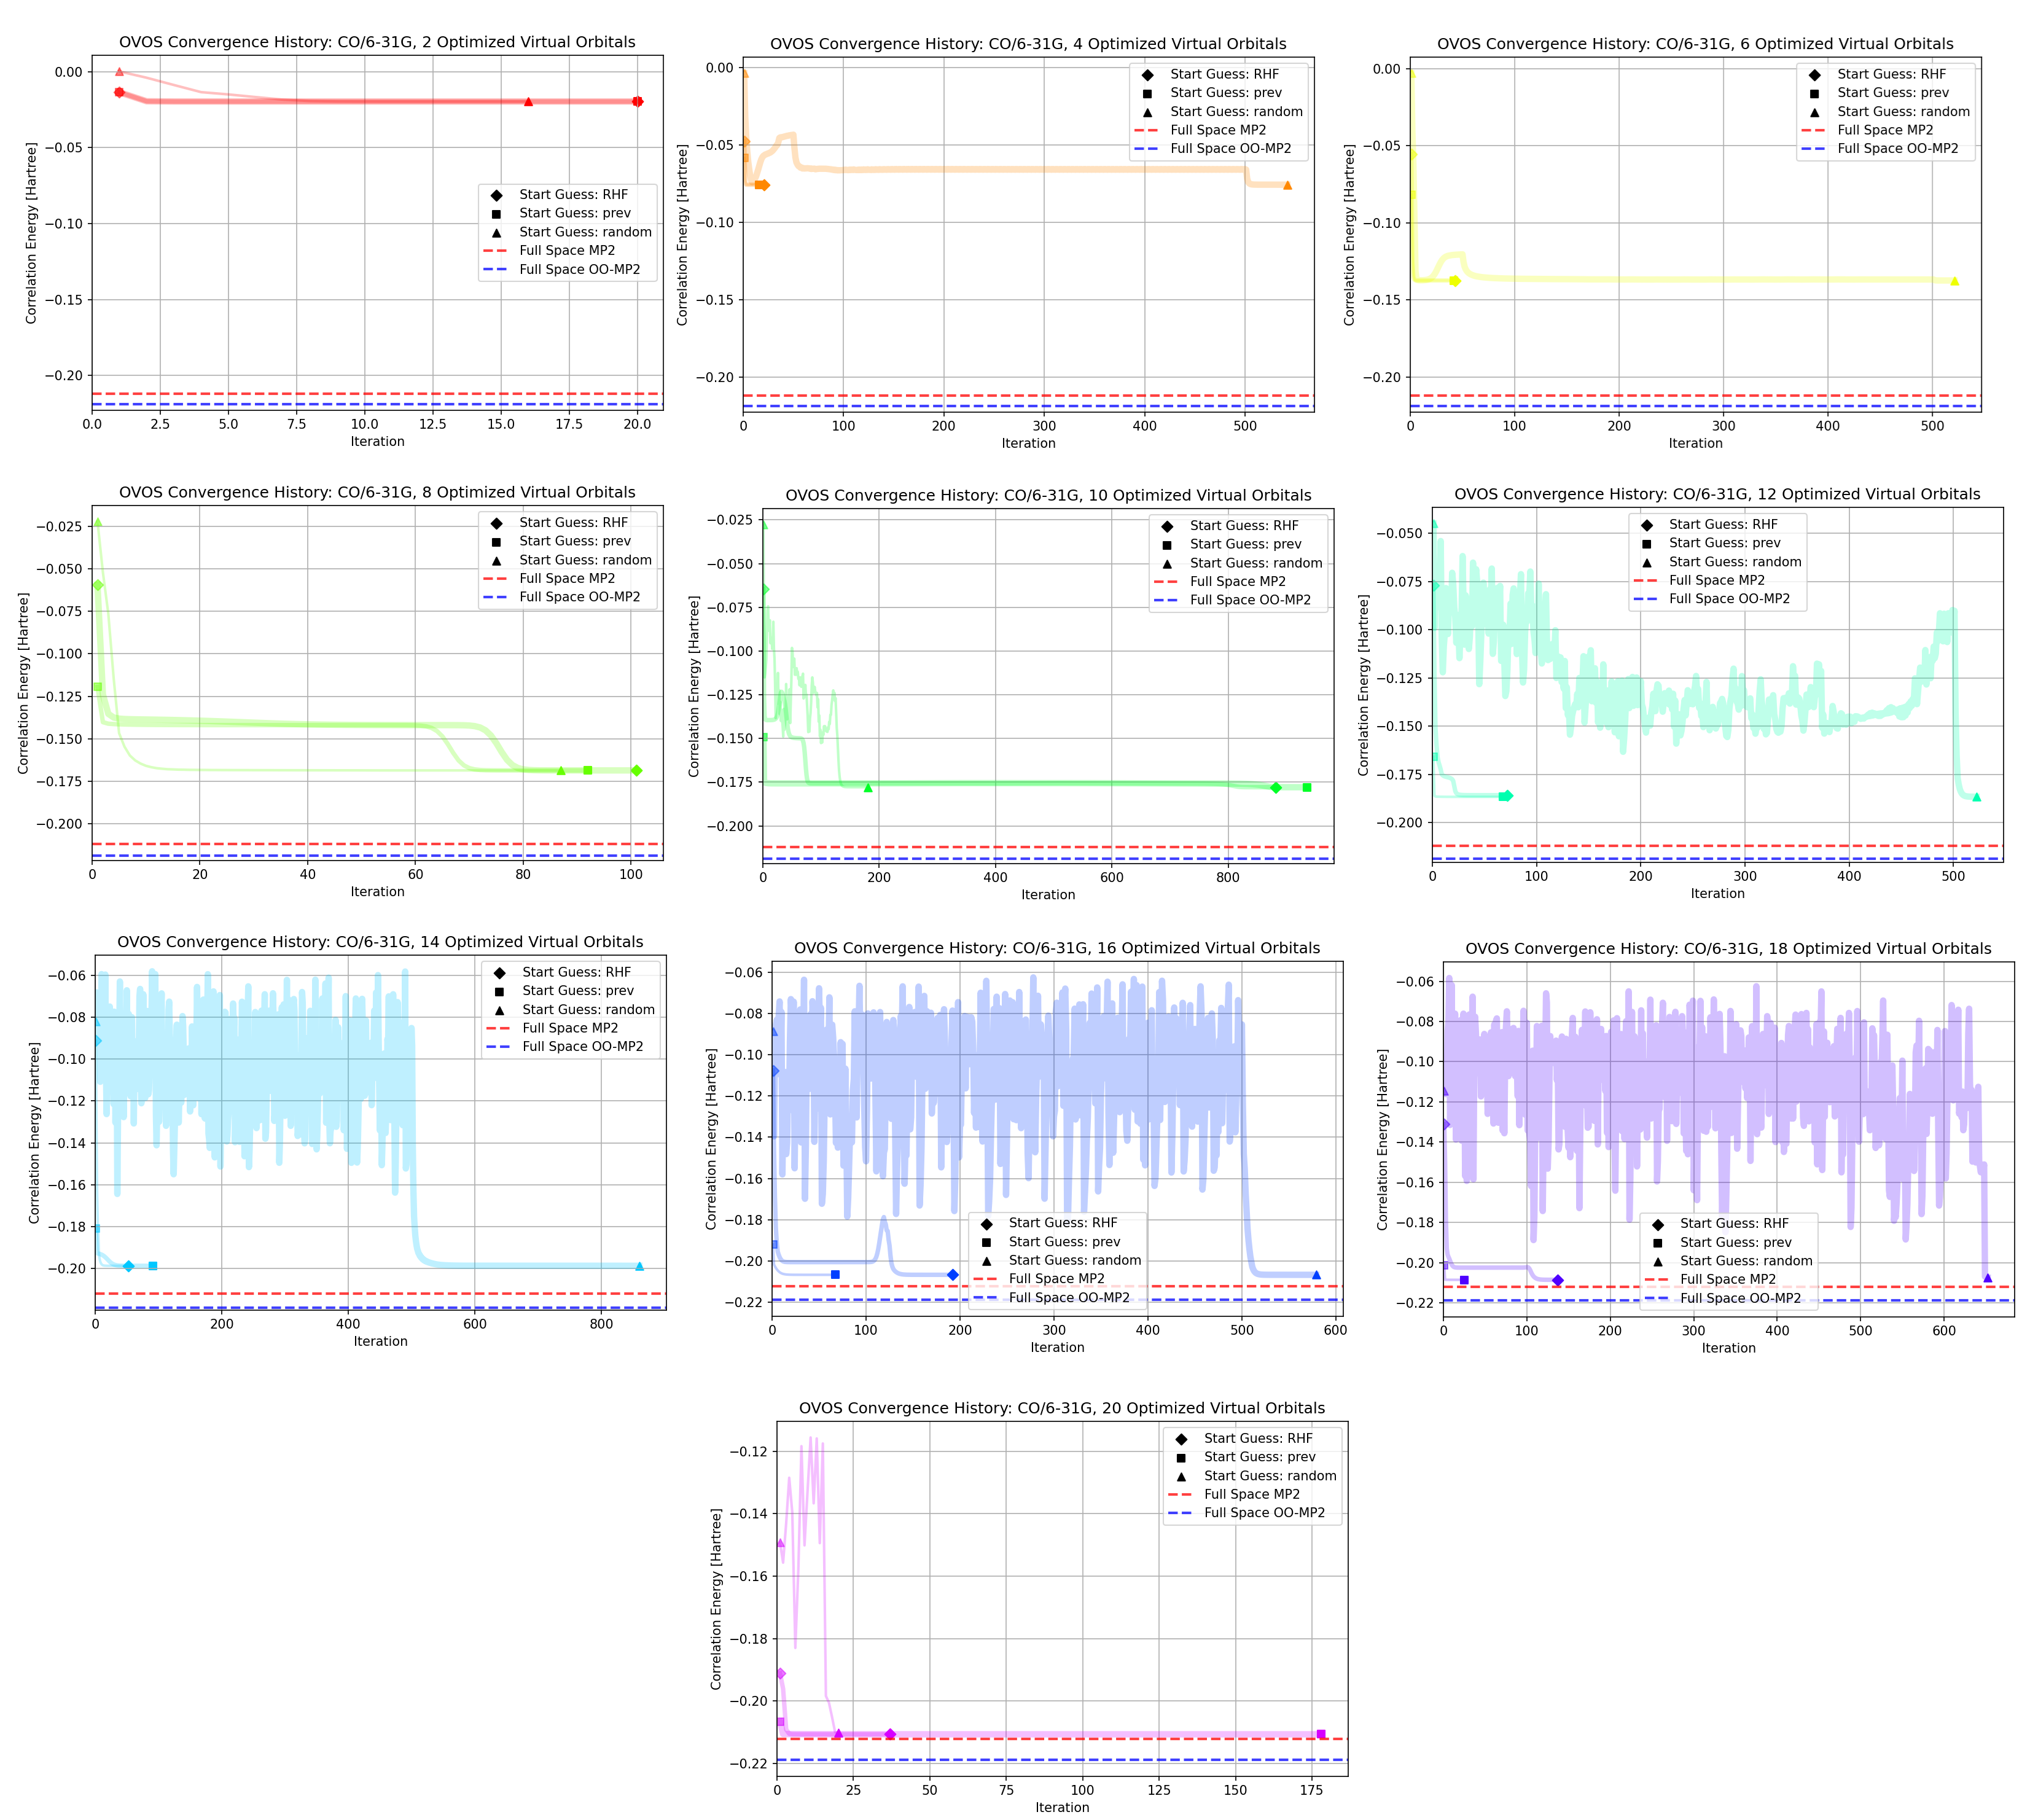
\includegraphics[width=0.75\textwidth]{figures/Ekstra/OVOS_conv_CO_6-31G.png}
    \caption{CO/6--31G OVOS convergence history for each active unoccupied orbitals, colour coded to fit the OVOS convergence plot in Figure~\ref{fig:appb_MP2_6-31G_ovos} and in Section~\ref{subsec:results_ovos_mp2}. The OVOS algorithm takes RHF (diamond), previous (square), and random (triangle) as start guesses. Dashed lines: full-space MP2 (red), OO-MP2 (blue), FCI (green) references.}
    \label{fig:appb_conv_CO_6-31G_ovos}
\end{figure}

\newpage

\begin{figure}[H]
    \centering
    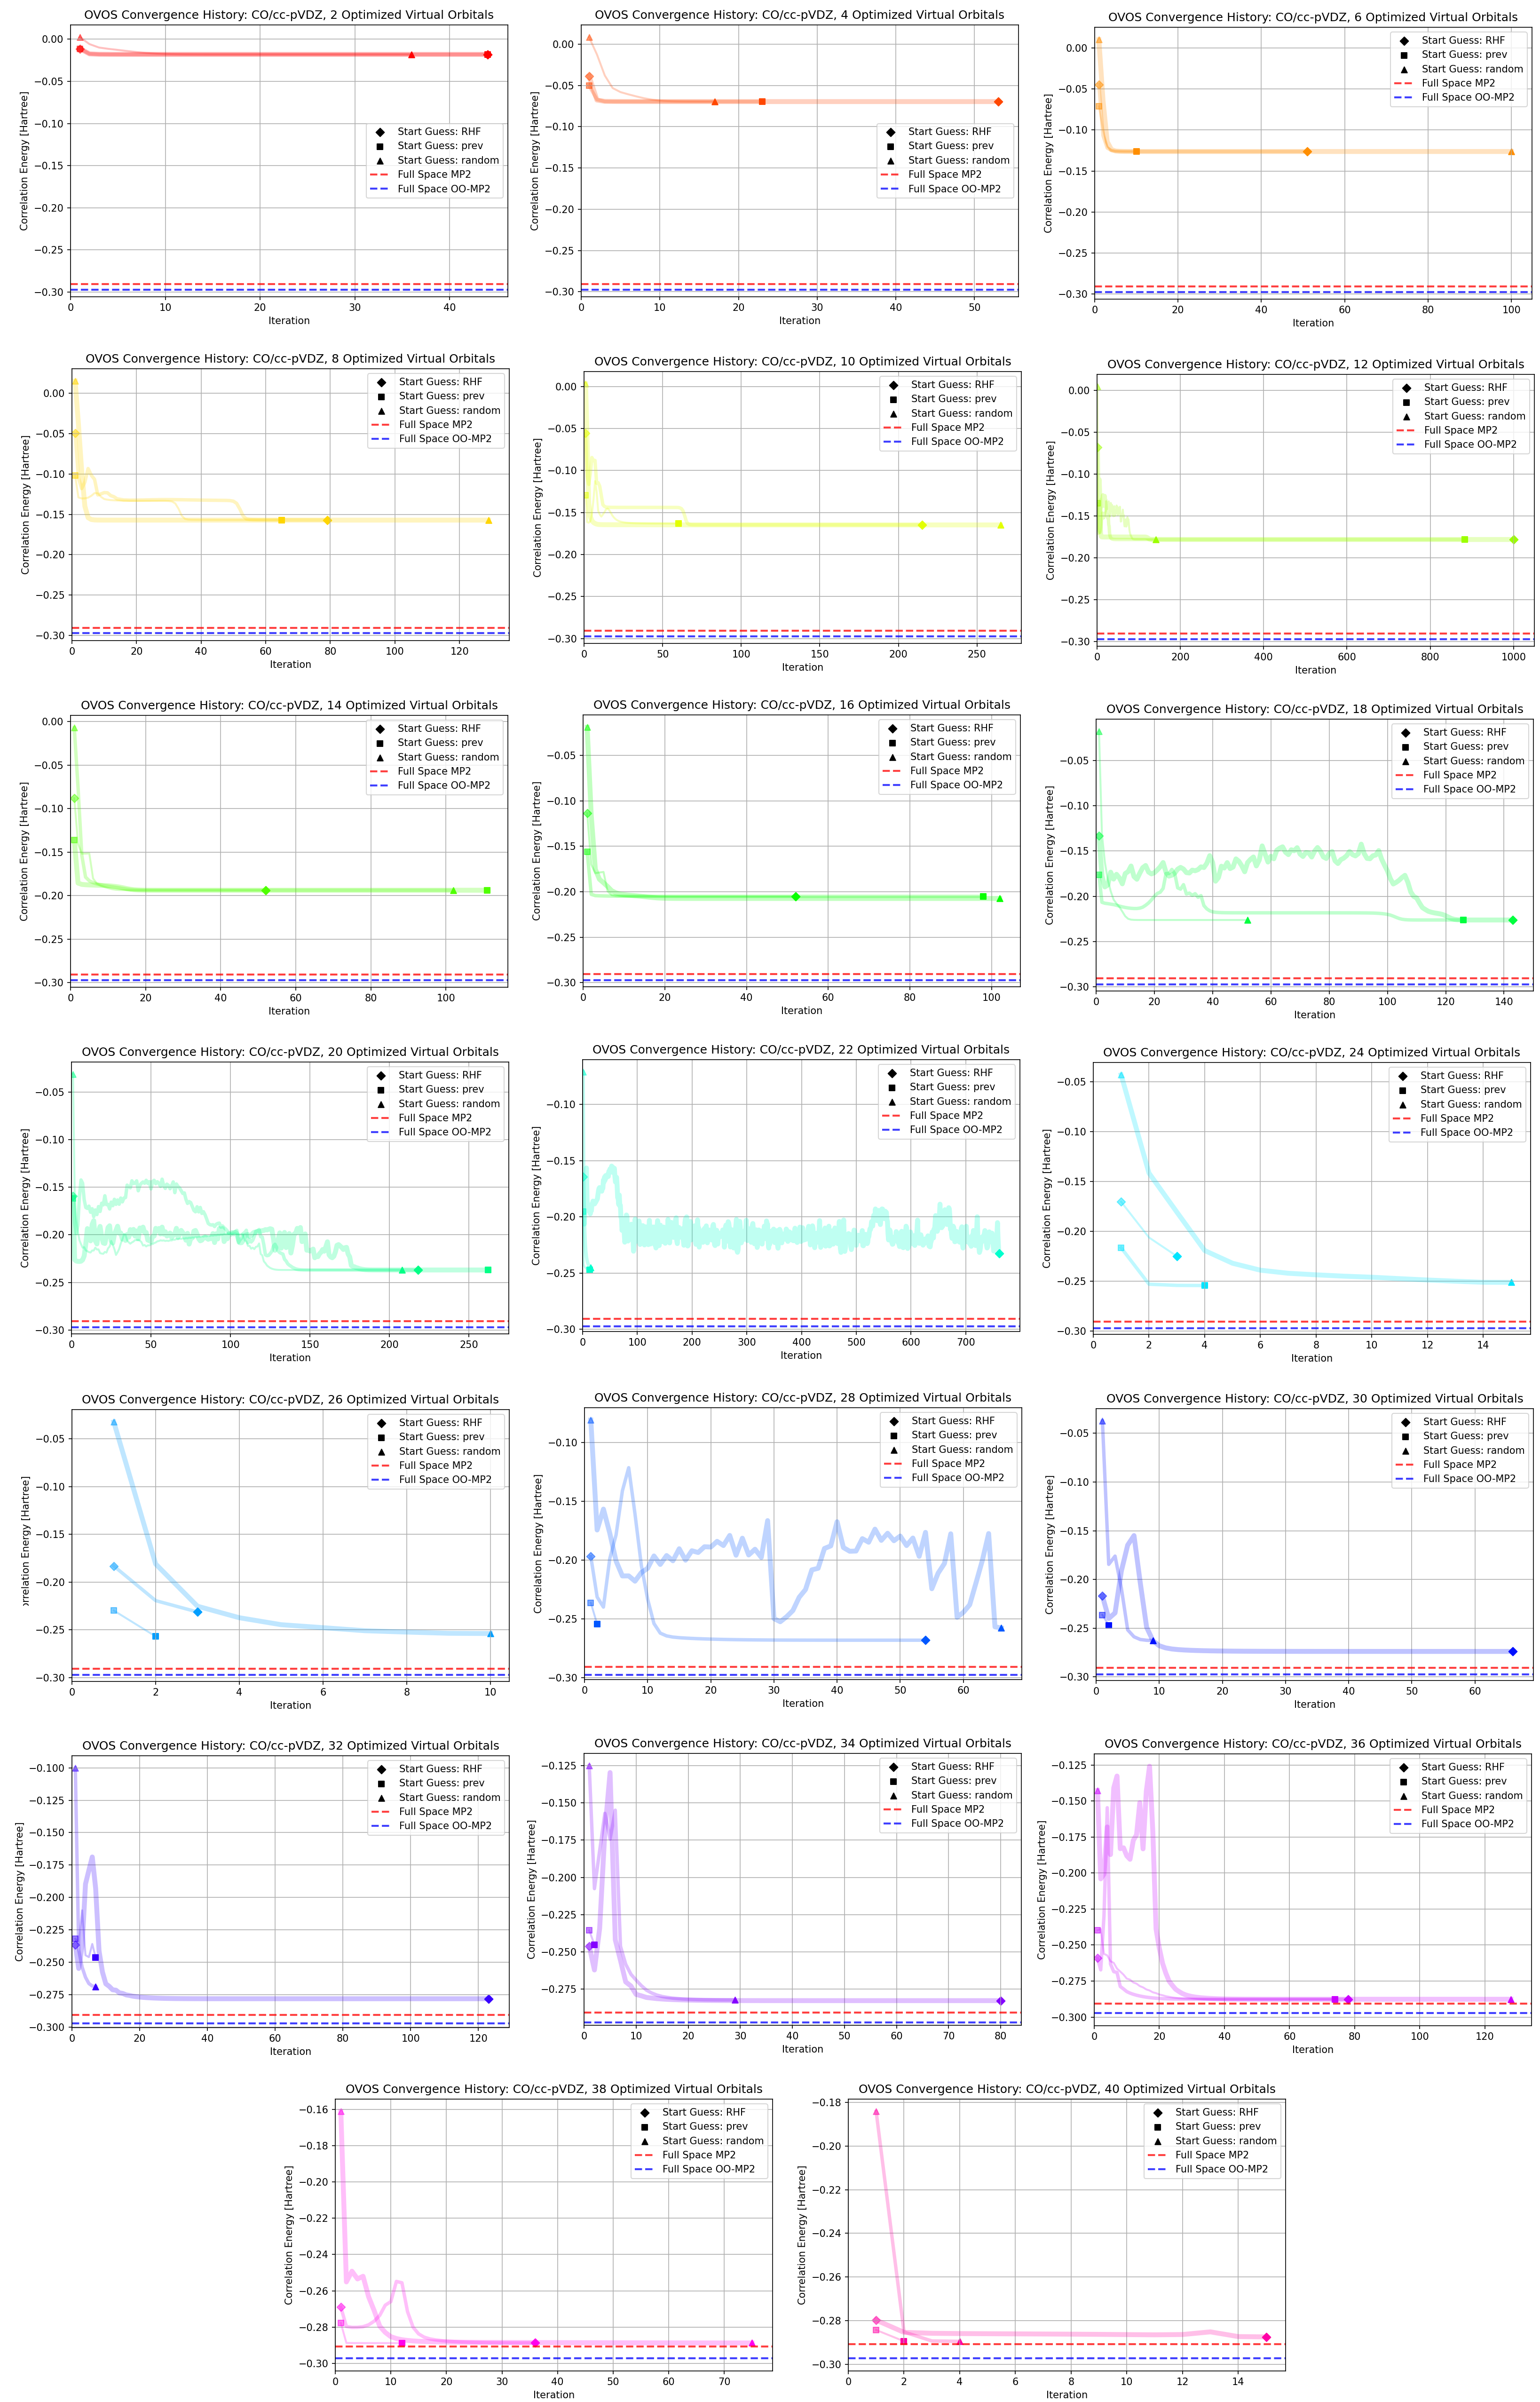
\includegraphics[width=0.9\textwidth]{figures/Ekstra/OVOS_conv_CO_cc-pVDZ.png}
    \caption{CO/cc--pVDZ OVOS convergence history for each active unoccupied orbitals, colour coded to fit the OVOS convergence plot in Figure~\ref{fig:appb_MP2_6-31G_ovos} and in Section~\ref{subsec:results_ovos_mp2}. The OVOS algorithm takes RHF (diamond), previous (square), and random (triangle) as start guesses. Dashed lines: full-space MP2 (red), OO-MP2 (blue), FCI (green) references.}
    \label{fig:appb_conv_CO_cc-pVDZ_ovos}
\end{figure}

\newpage

\begin{figure}[H]
    \centering
    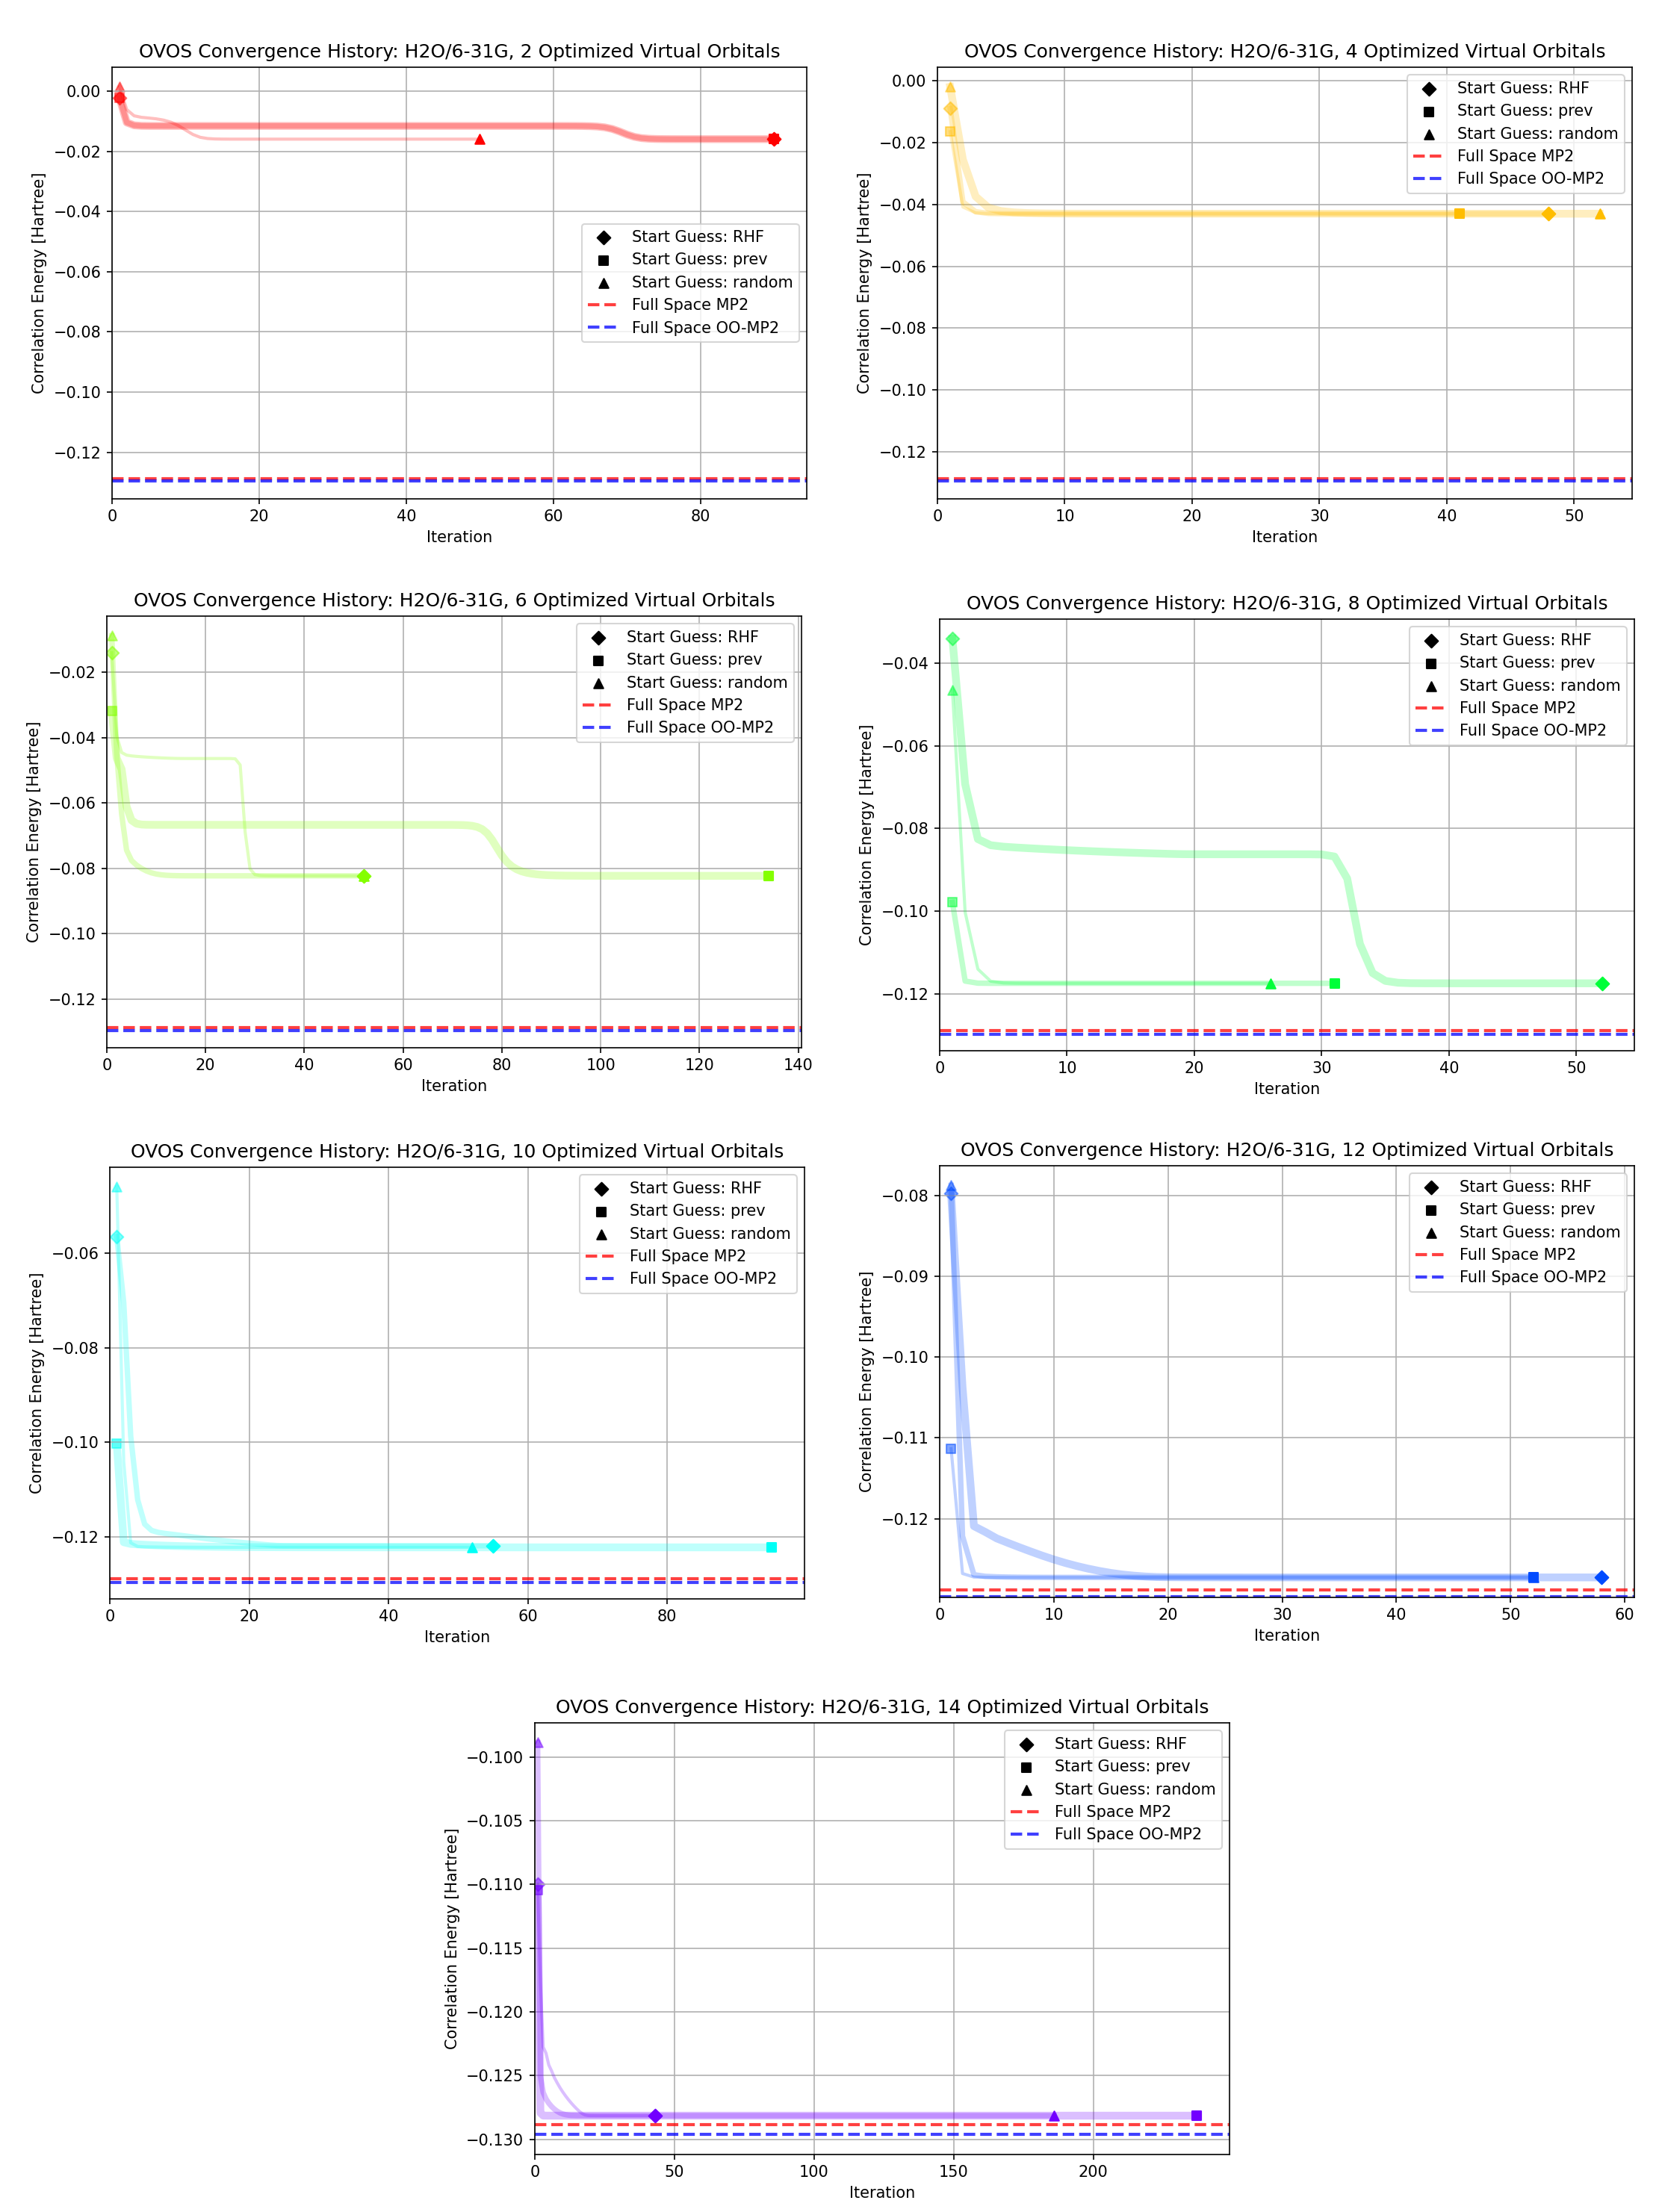
\includegraphics[width=0.9\textwidth]{figures/Ekstra/OVOS_conv_H2O_6-31G.png}
    \caption{H$_2$O/6--31G OVOS convergence history for each active unoccupied orbitals, colour coded to fit the OVOS convergence plot in Figure~\ref{fig:appb_MP2_6-31G_ovos} and in Section~\ref{subsec:results_ovos_mp2}. The OVOS algorithm takes RHF (diamond), previous (square), and random (triangle) as start guesses. Dashed lines: full-space MP2 (red), OO-MP2 (blue), FCI (green) references.}
    \label{fig:appb_conv_H2O_6-31G_ovos}
\end{figure}

\newpage

\begin{figure}[H]
    \centering
    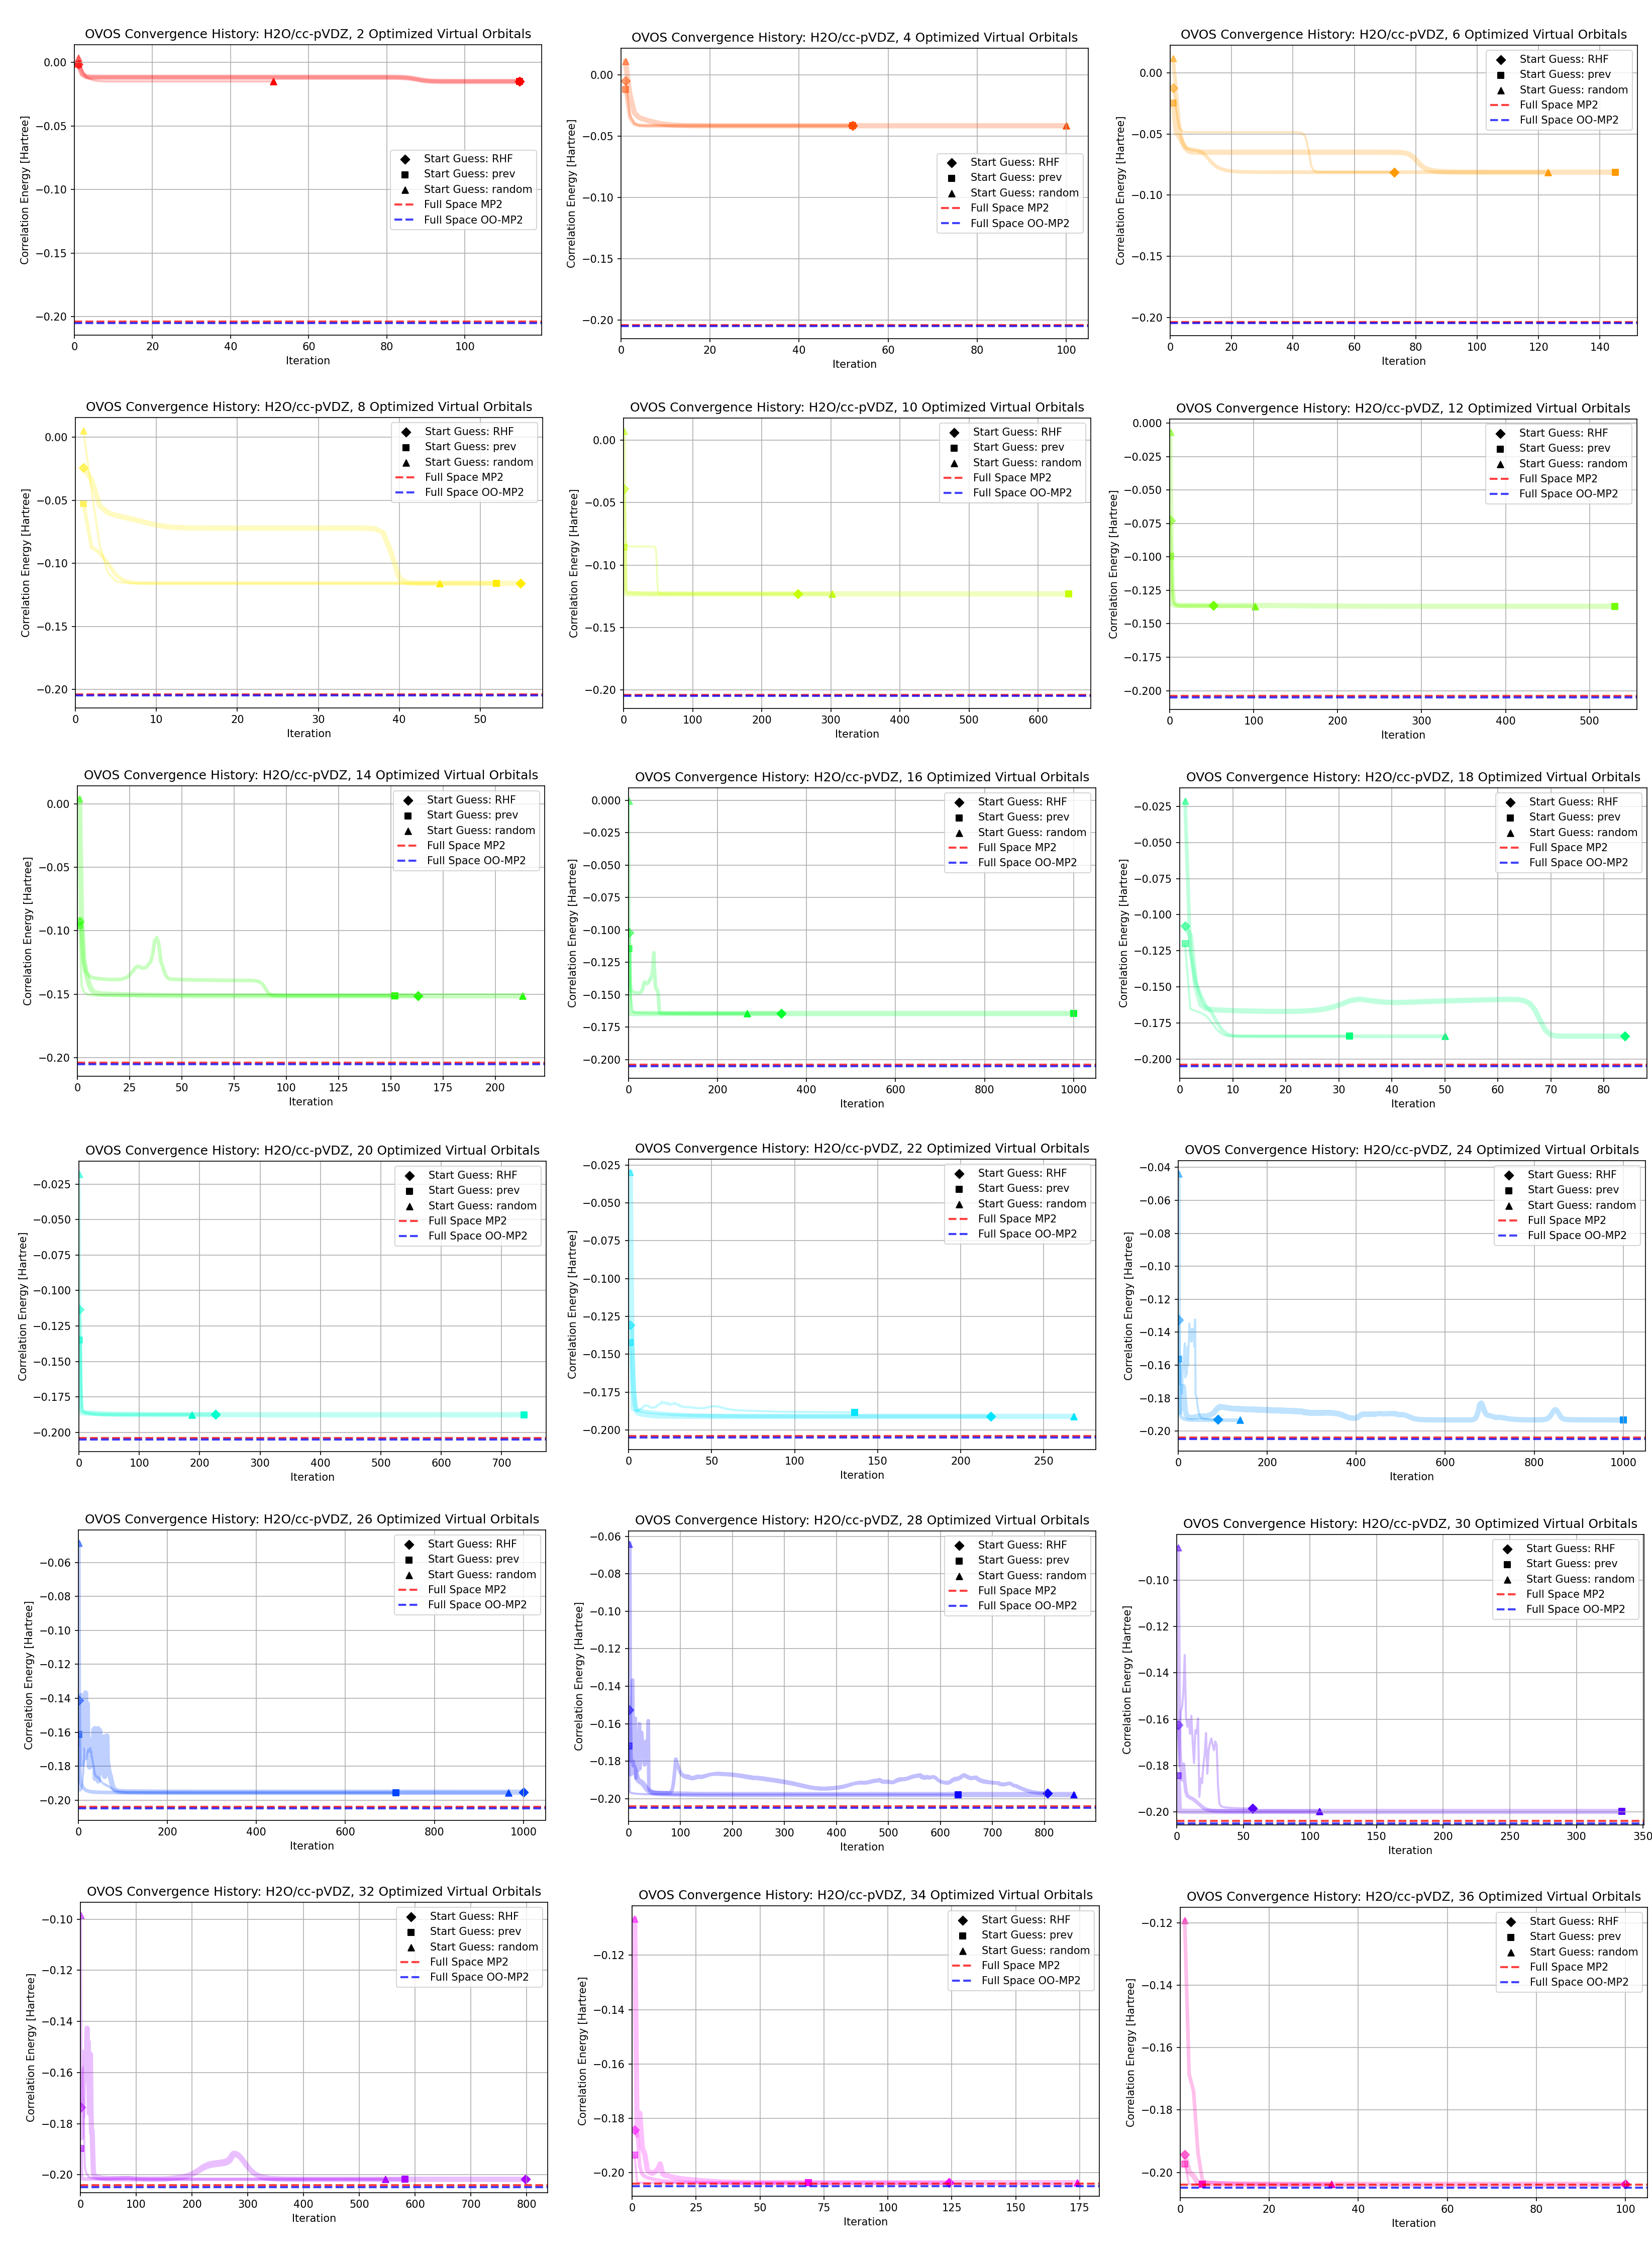
\includegraphics[width=0.9\textwidth]{figures/Ekstra/OVOS_conv_H2O_cc-pVDZ.png}
    \caption{H$_2$O/cc--pVDZ OVOS convergence history for each active unoccupied orbitals, colour coded to fit the OVOS convergence plot in Figure~\ref{fig:appb_MP2_6-31G_ovos} and in Section~\ref{subsec:results_ovos_mp2}. The OVOS algorithm takes RHF (diamond), previous (square), and random (triangle) as start guesses. Dashed lines: full-space MP2 (red), OO-MP2 (blue), FCI (green) references.}
    \label{fig:appb_conv_H2O_cc-pVDZ_ovos}
\end{figure}

\newpage

\begin{figure}[H]
    \centering
    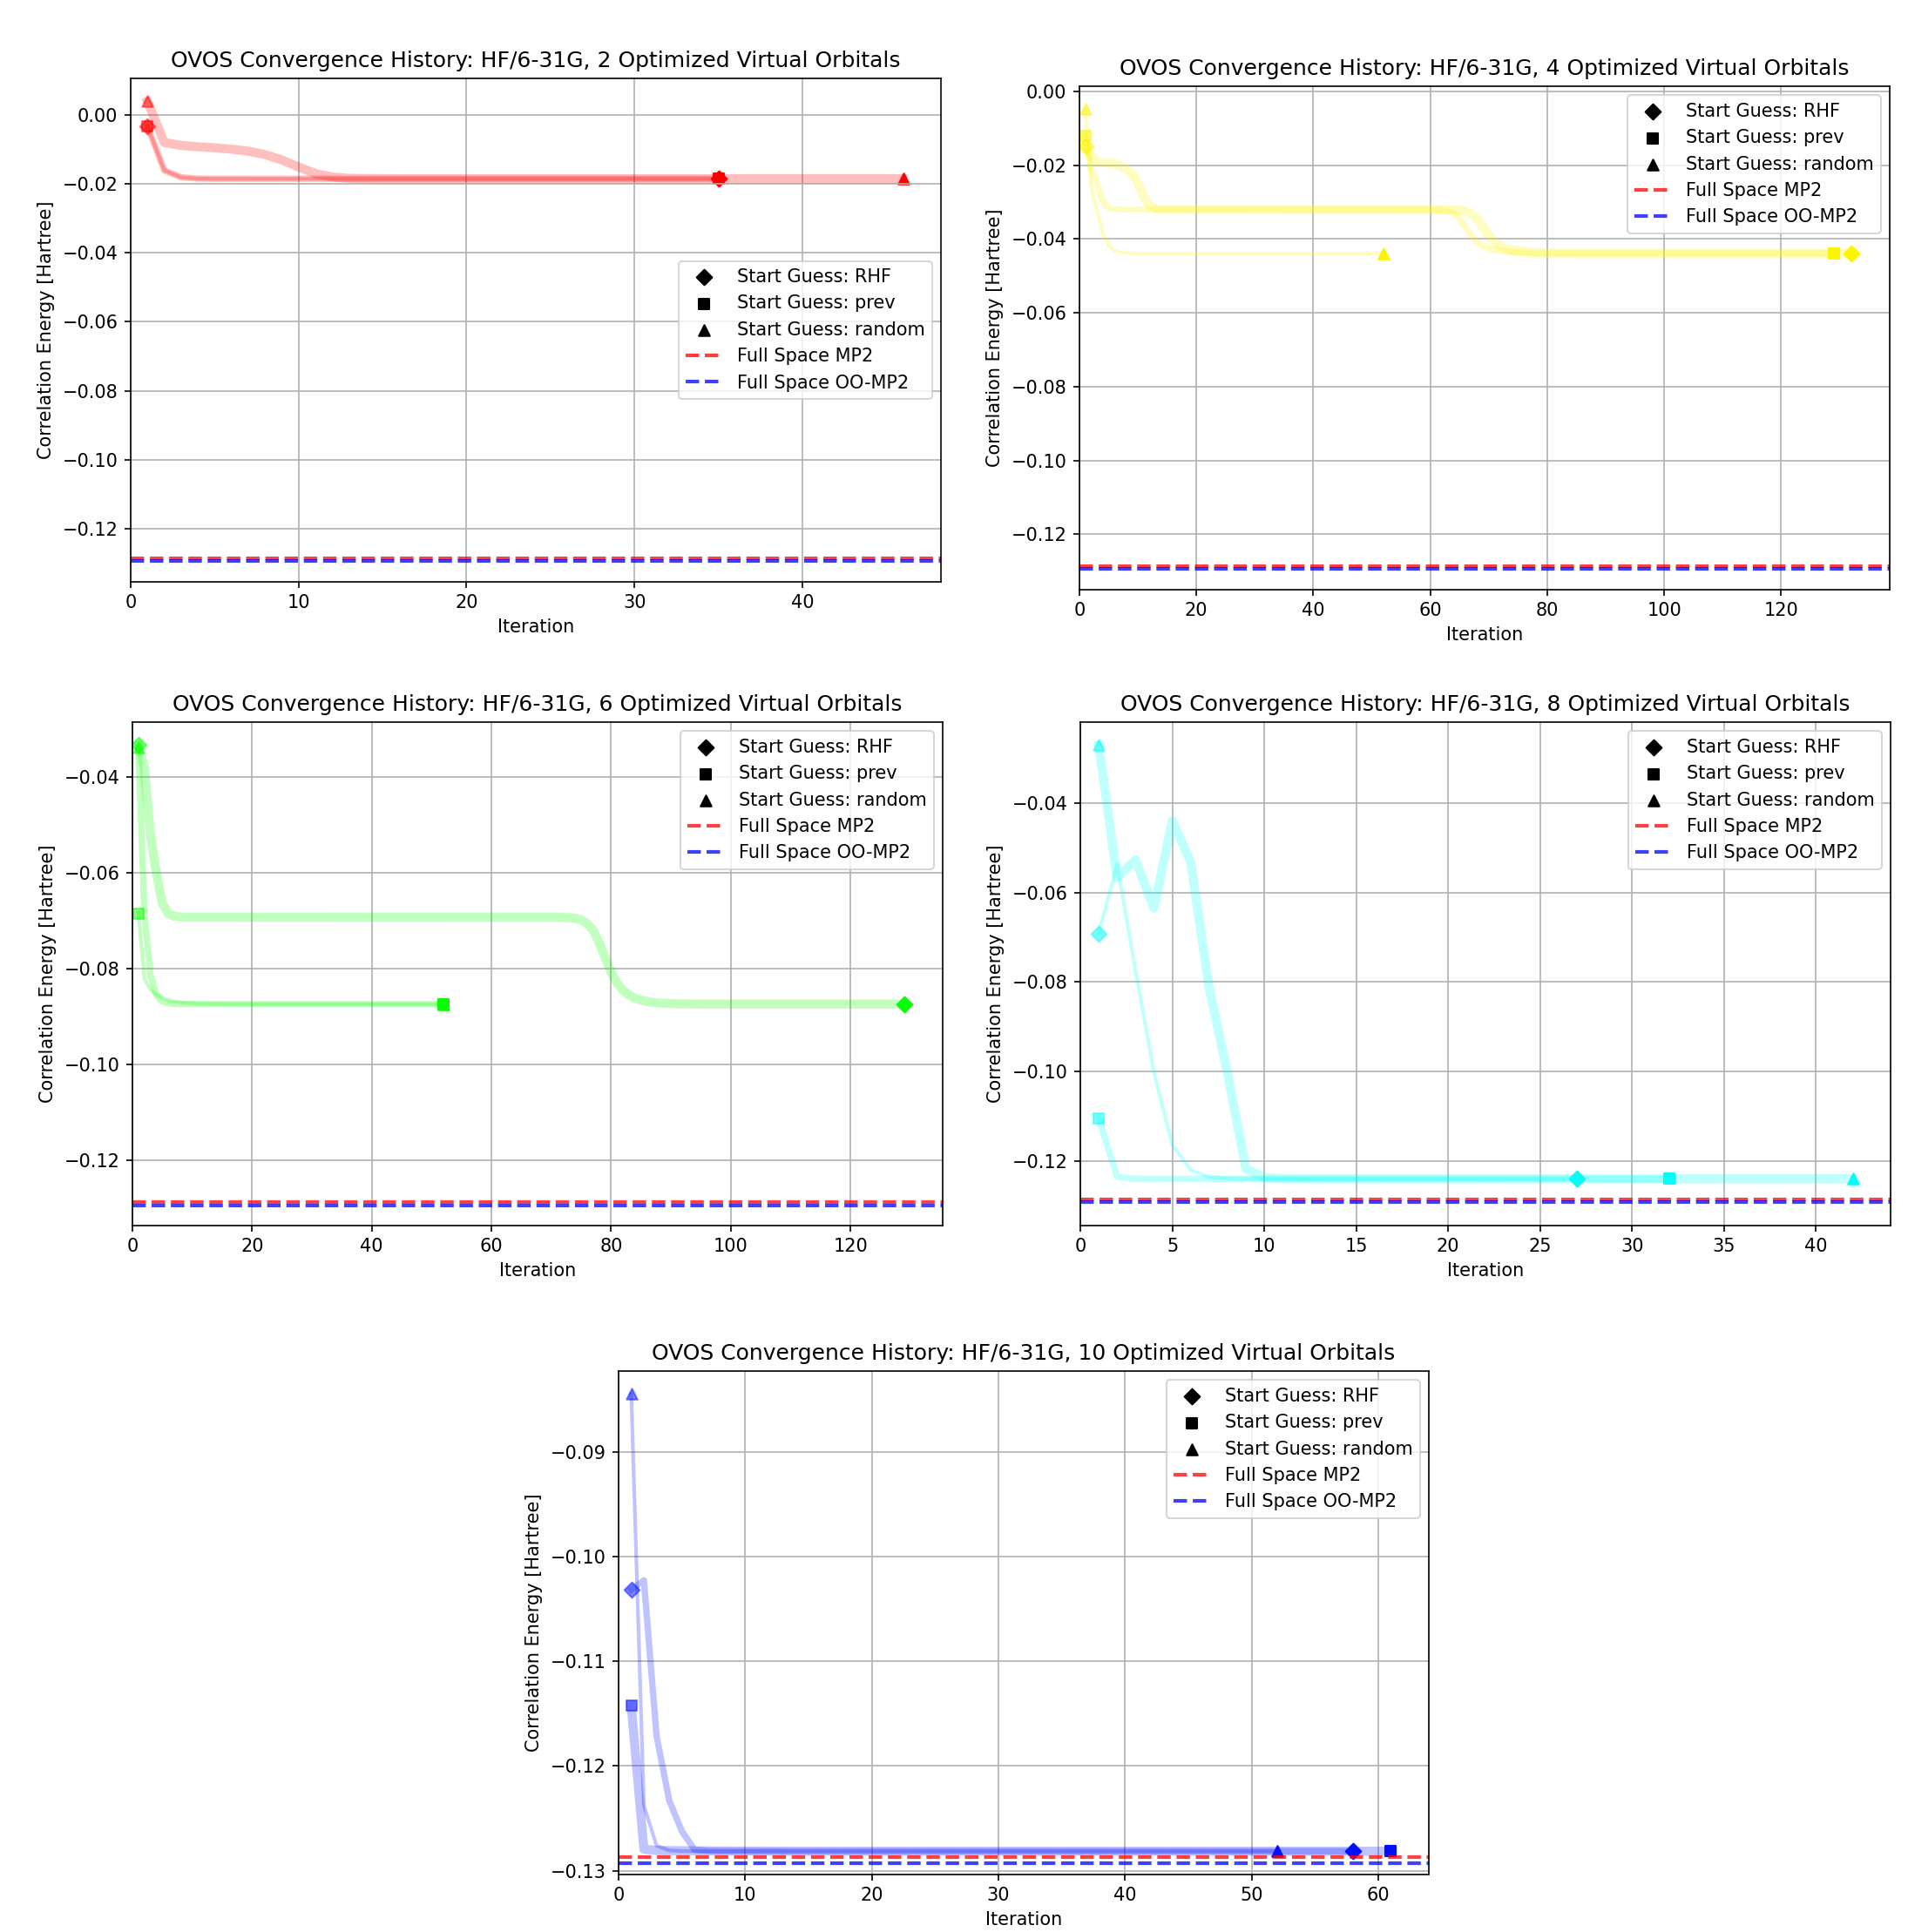
\includegraphics[width=0.9\textwidth]{figures/Ekstra/OVOS_conv_HF_6-31G.png}
    \caption{HF/6--31G OVOS convergence history for each active unoccupied orbitals, colour coded to fit the OVOS convergence plot in Figure~\ref{fig:appb_MP2_6-31G_ovos} and in Section~\ref{subsec:results_ovos_mp2}. The OVOS algorithm takes RHF (diamond), previous (square), and random (triangle) as start guesses. Dashed lines: full-space MP2 (red), OO-MP2 (blue), FCI (green) references.}
    \label{fig:appb_conv_HF_6-31G_ovos}
\end{figure}

\newpage

\begin{figure}[H]
    \centering
    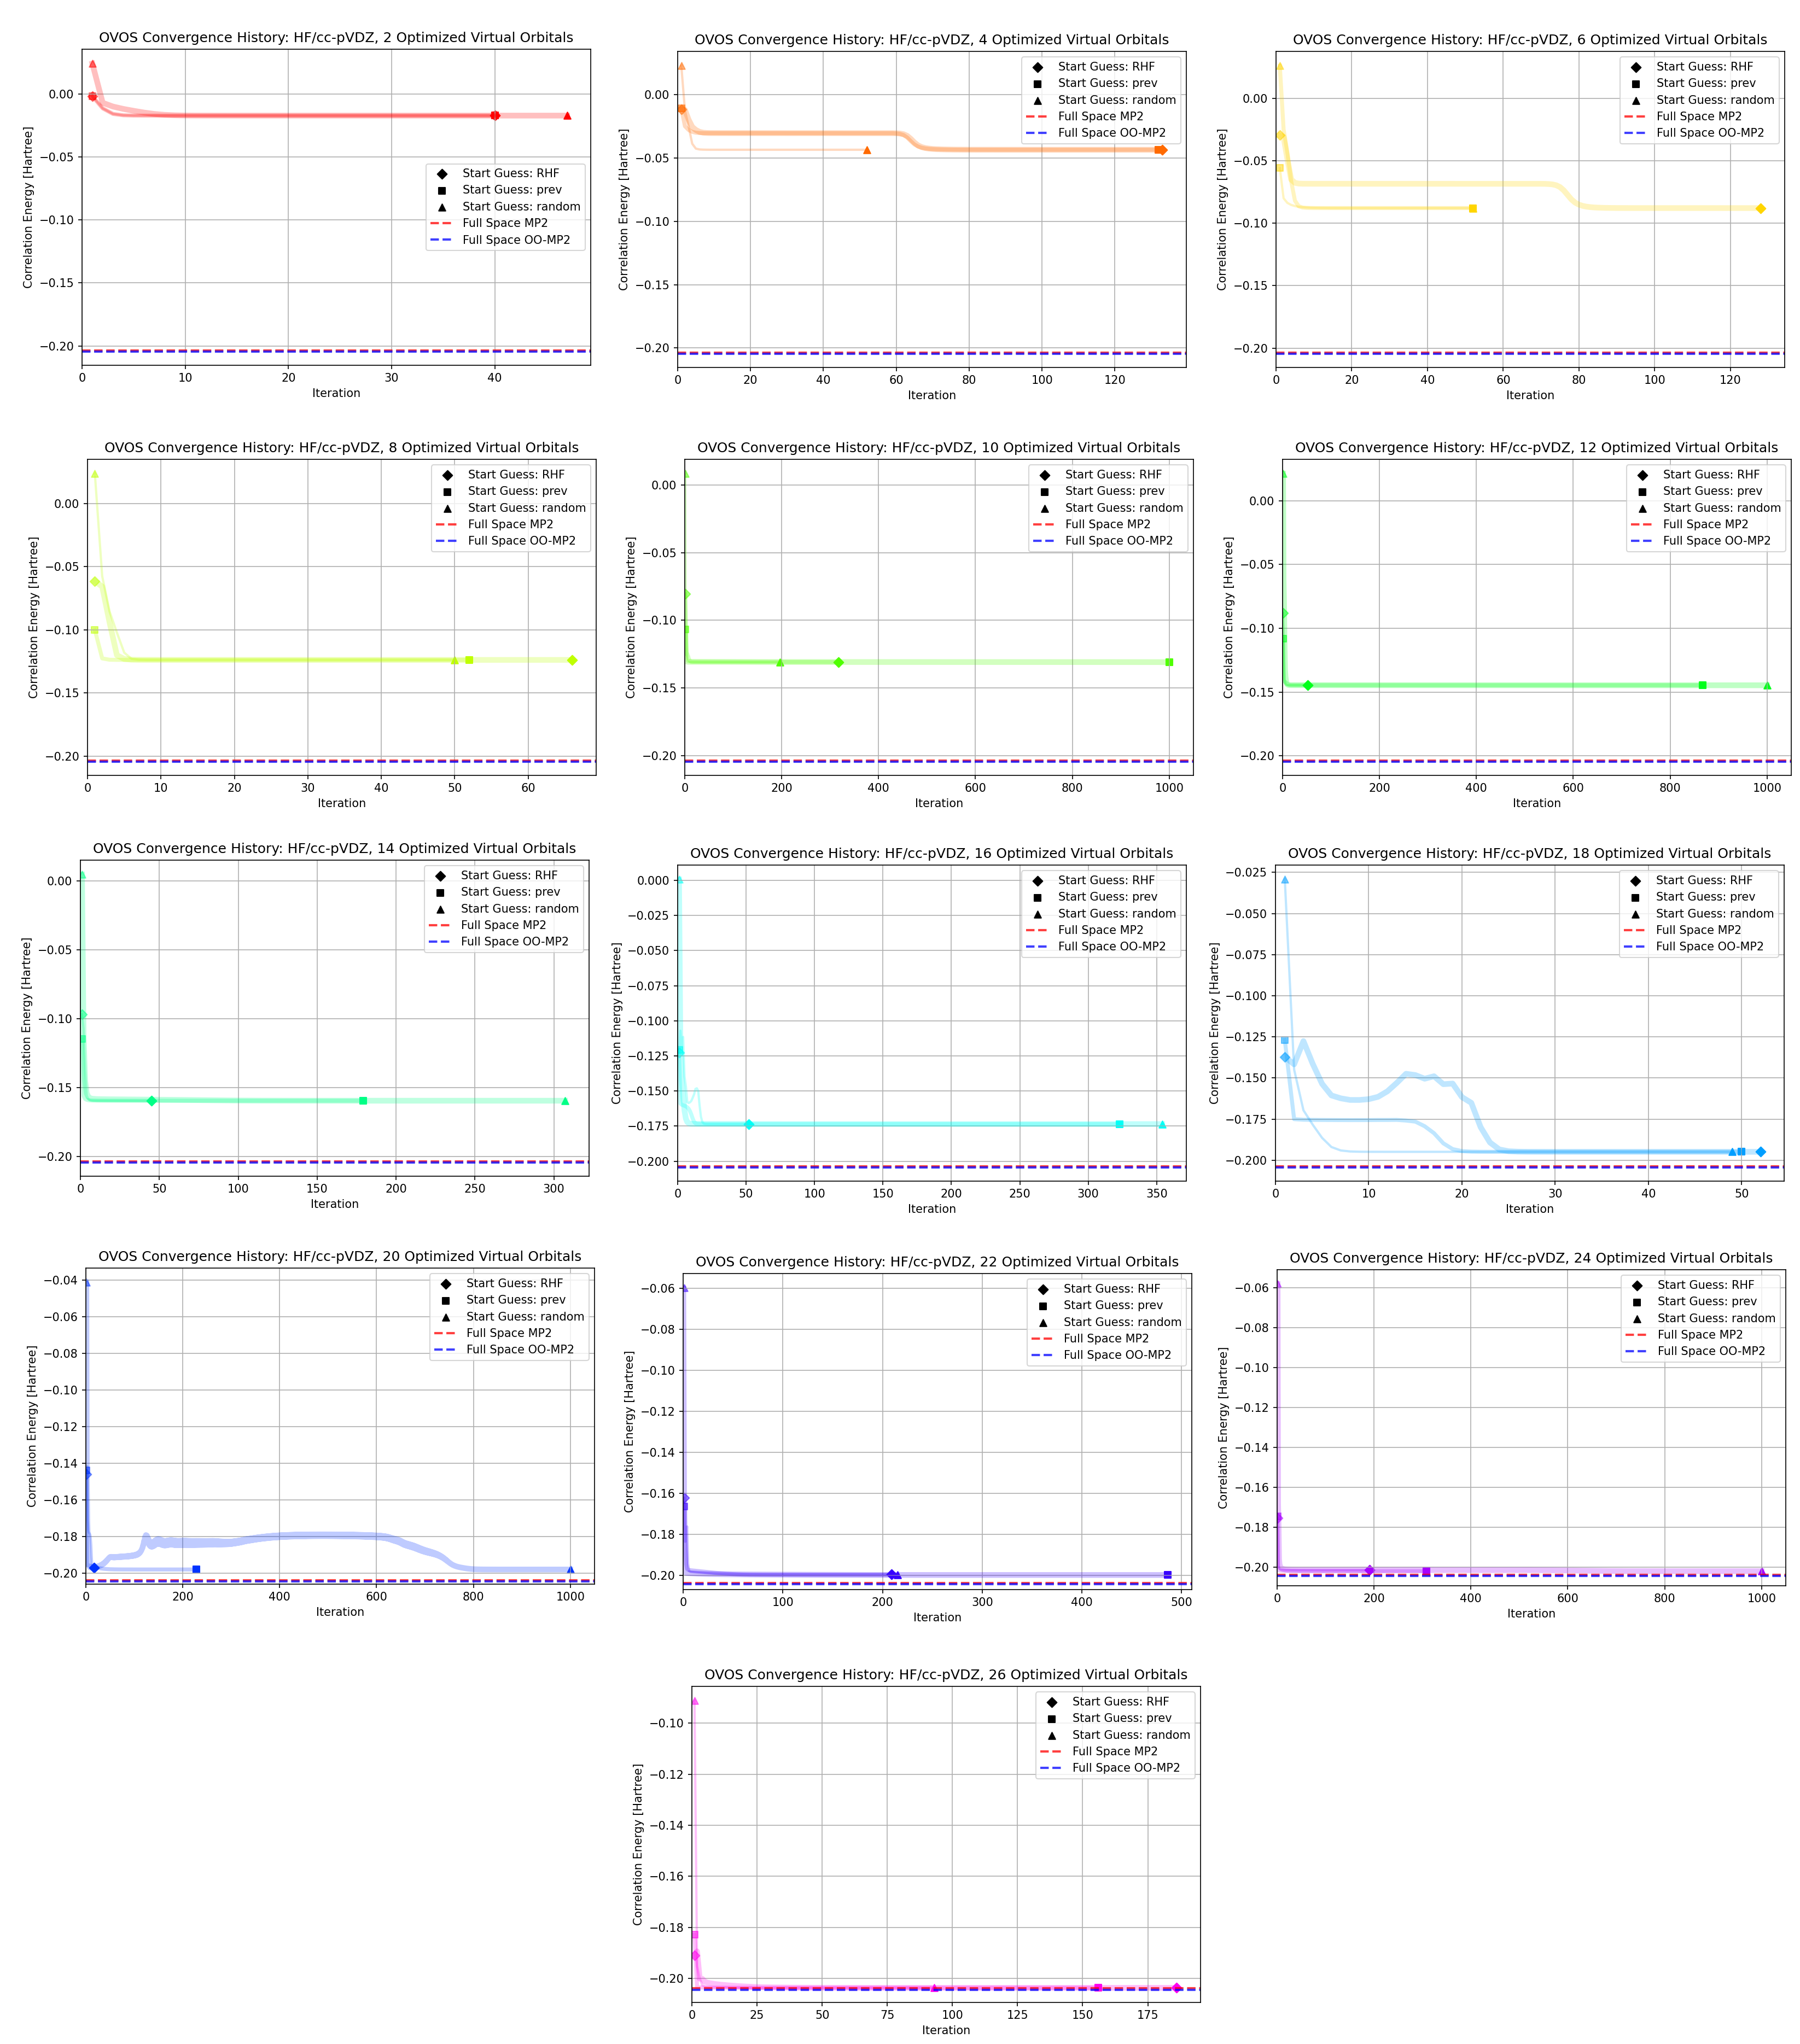
\includegraphics[width=0.9\textwidth]{figures/Ekstra/OVOS_conv_HF_cc-pVDZ.png}
    \caption{HF/cc--pVDZ OVOS convergence history for each active unoccupied orbitals, colour coded to fit the OVOS convergence plot in Figure~\ref{fig:appb_MP2_6-31G_ovos} and in Section~\ref{subsec:results_ovos_mp2}. The OVOS algorithm takes RHF (diamond), previous (square), and random (triangle) as start guesses. Dashed lines: full-space MP2 (red), OO-MP2 (blue), FCI (green) references.}
    \label{fig:appb_conv_HF_cc-pVDZ_ovos}
\end{figure}

\newpage

\begin{figure}[H]
    \centering
    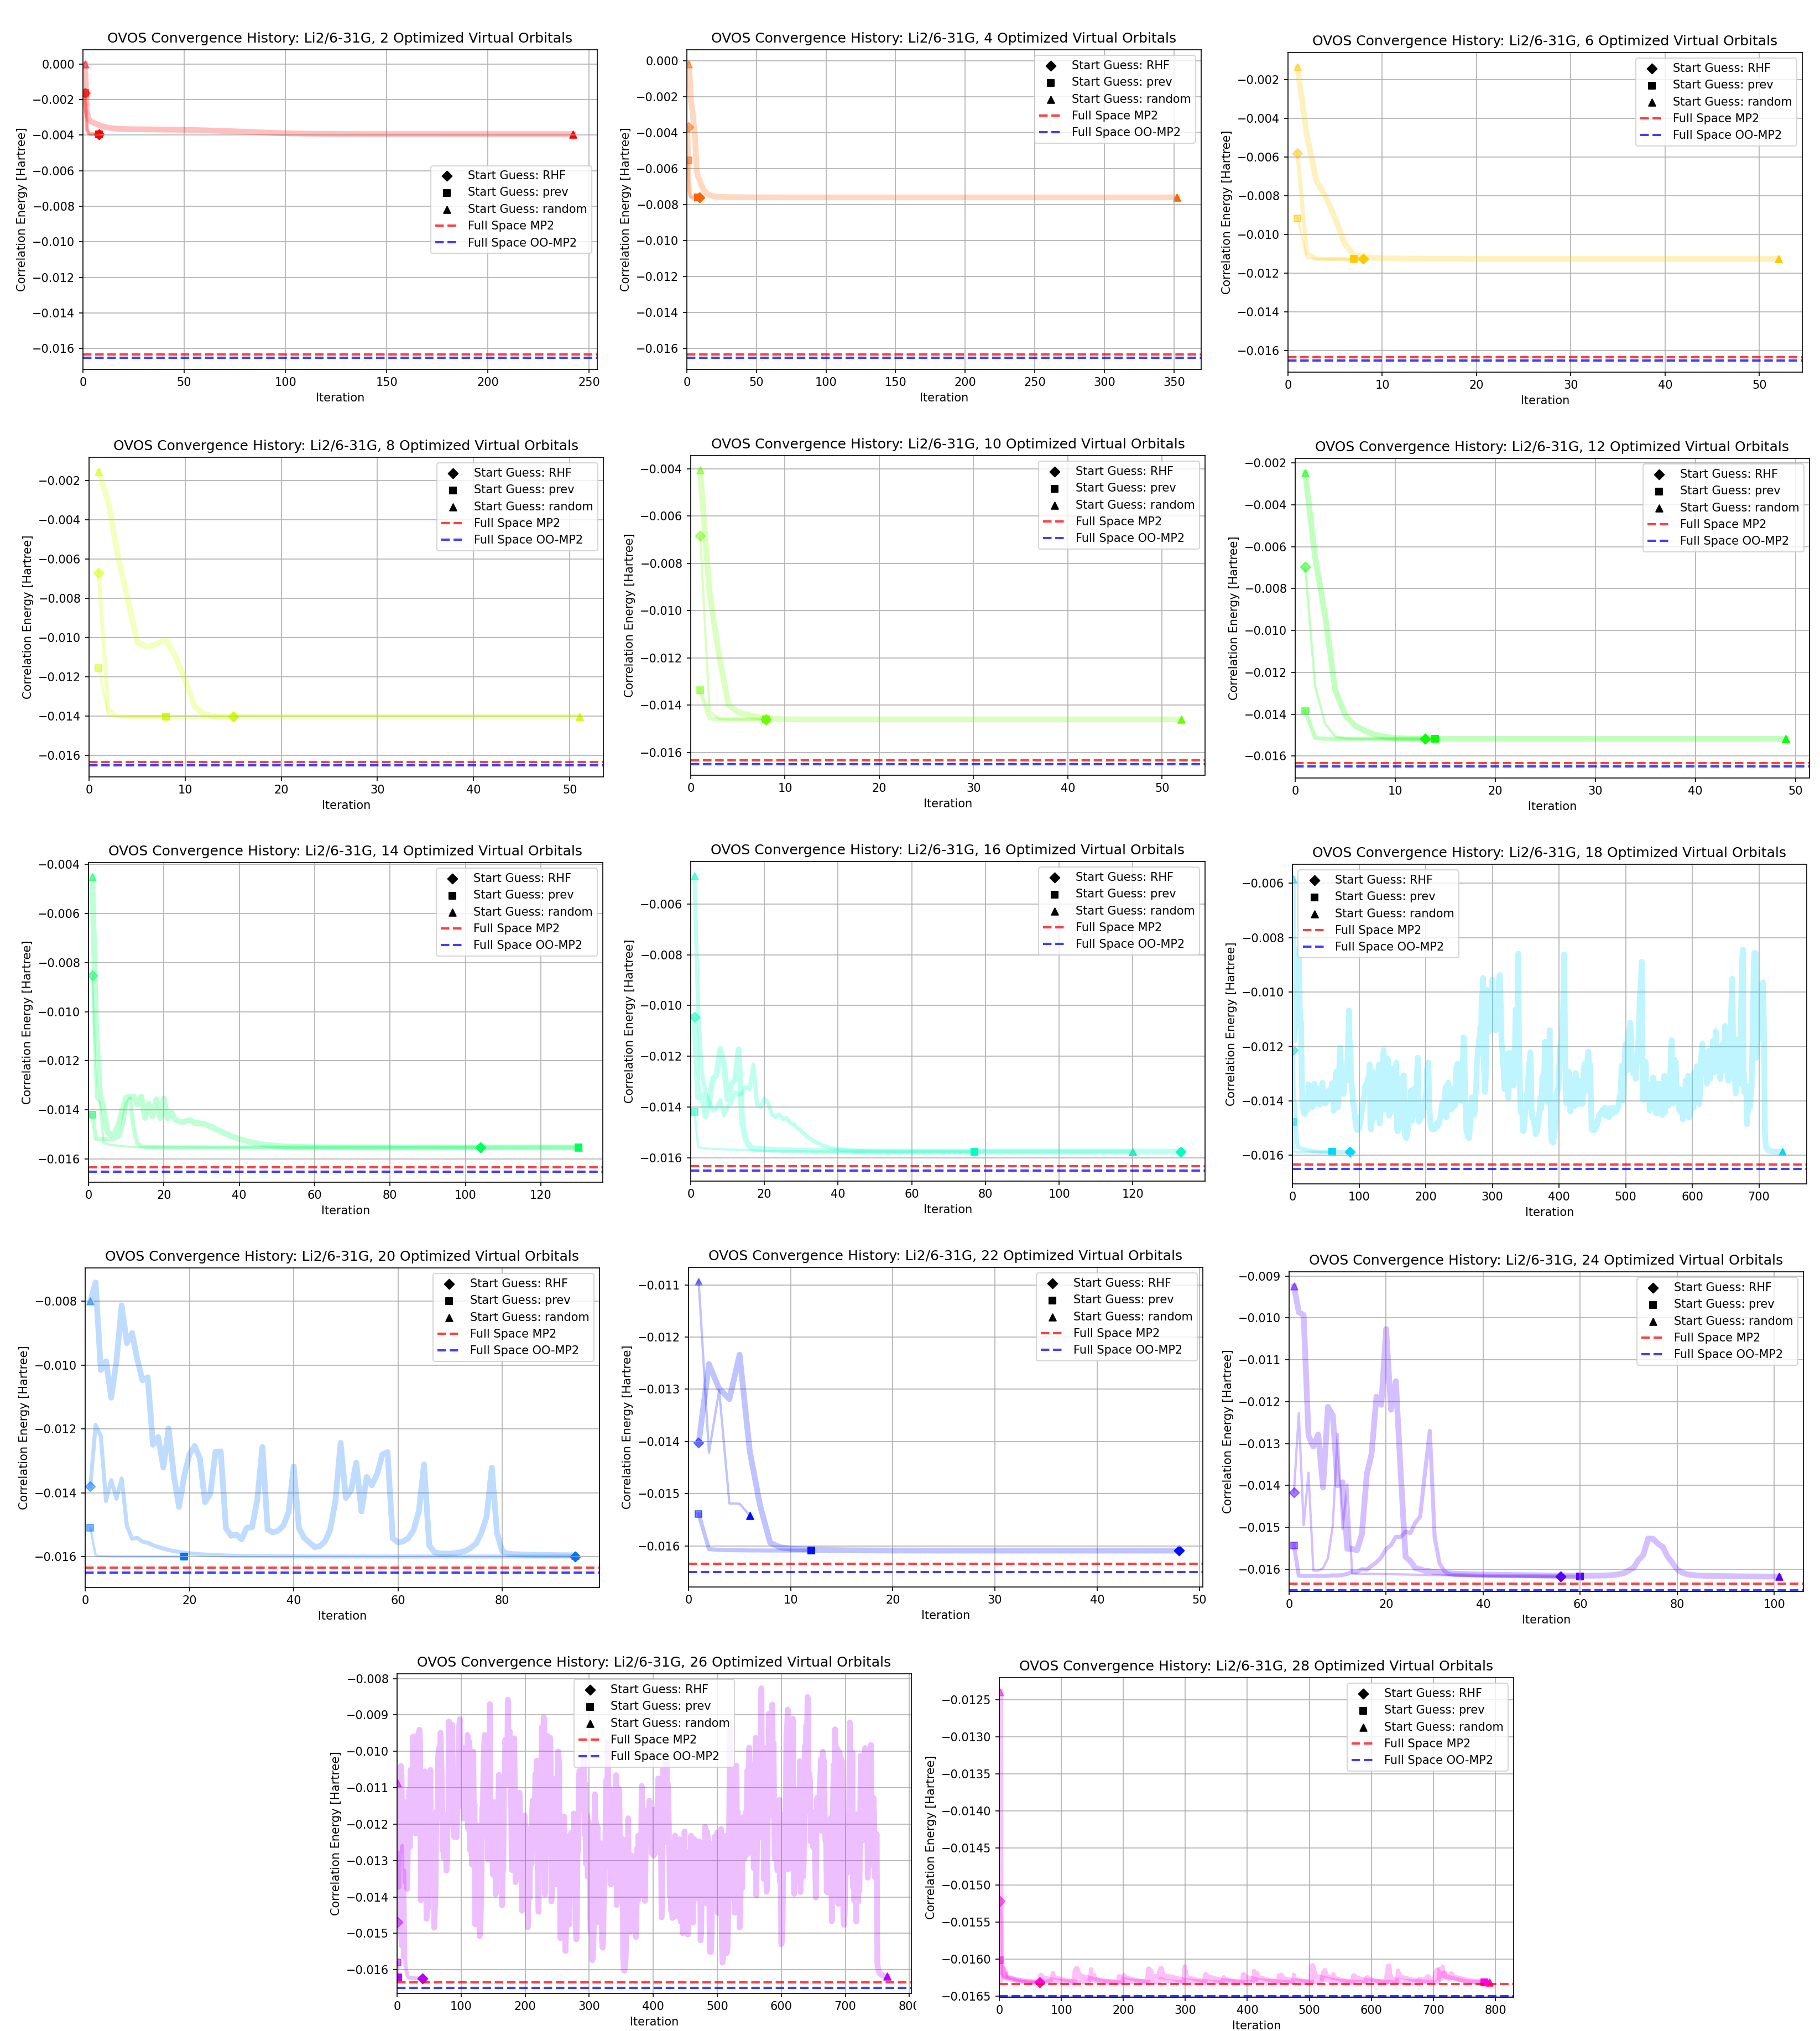
\includegraphics[width=0.9\textwidth]{figures/Ekstra/OVOS_conv_Li2_6-31G.png}
    \caption{Li$_2$/6--31G OVOS convergence history for each active unoccupied orbitals, colour coded to fit the OVOS convergence plot in Figure~\ref{fig:appb_MP2_6-31G_ovos} and in Section~\ref{subsec:results_ovos_mp2}. The OVOS algorithm takes RHF (diamond), previous (square), and random (triangle) as start guesses. Dashed lines: full-space MP2 (red), OO-MP2 (blue), FCI (green) references.}
    \label{fig:appb_conv_Li2_6-31G_ovos}
\end{figure}

\newpage

\begin{figure}[H]
    \centering
    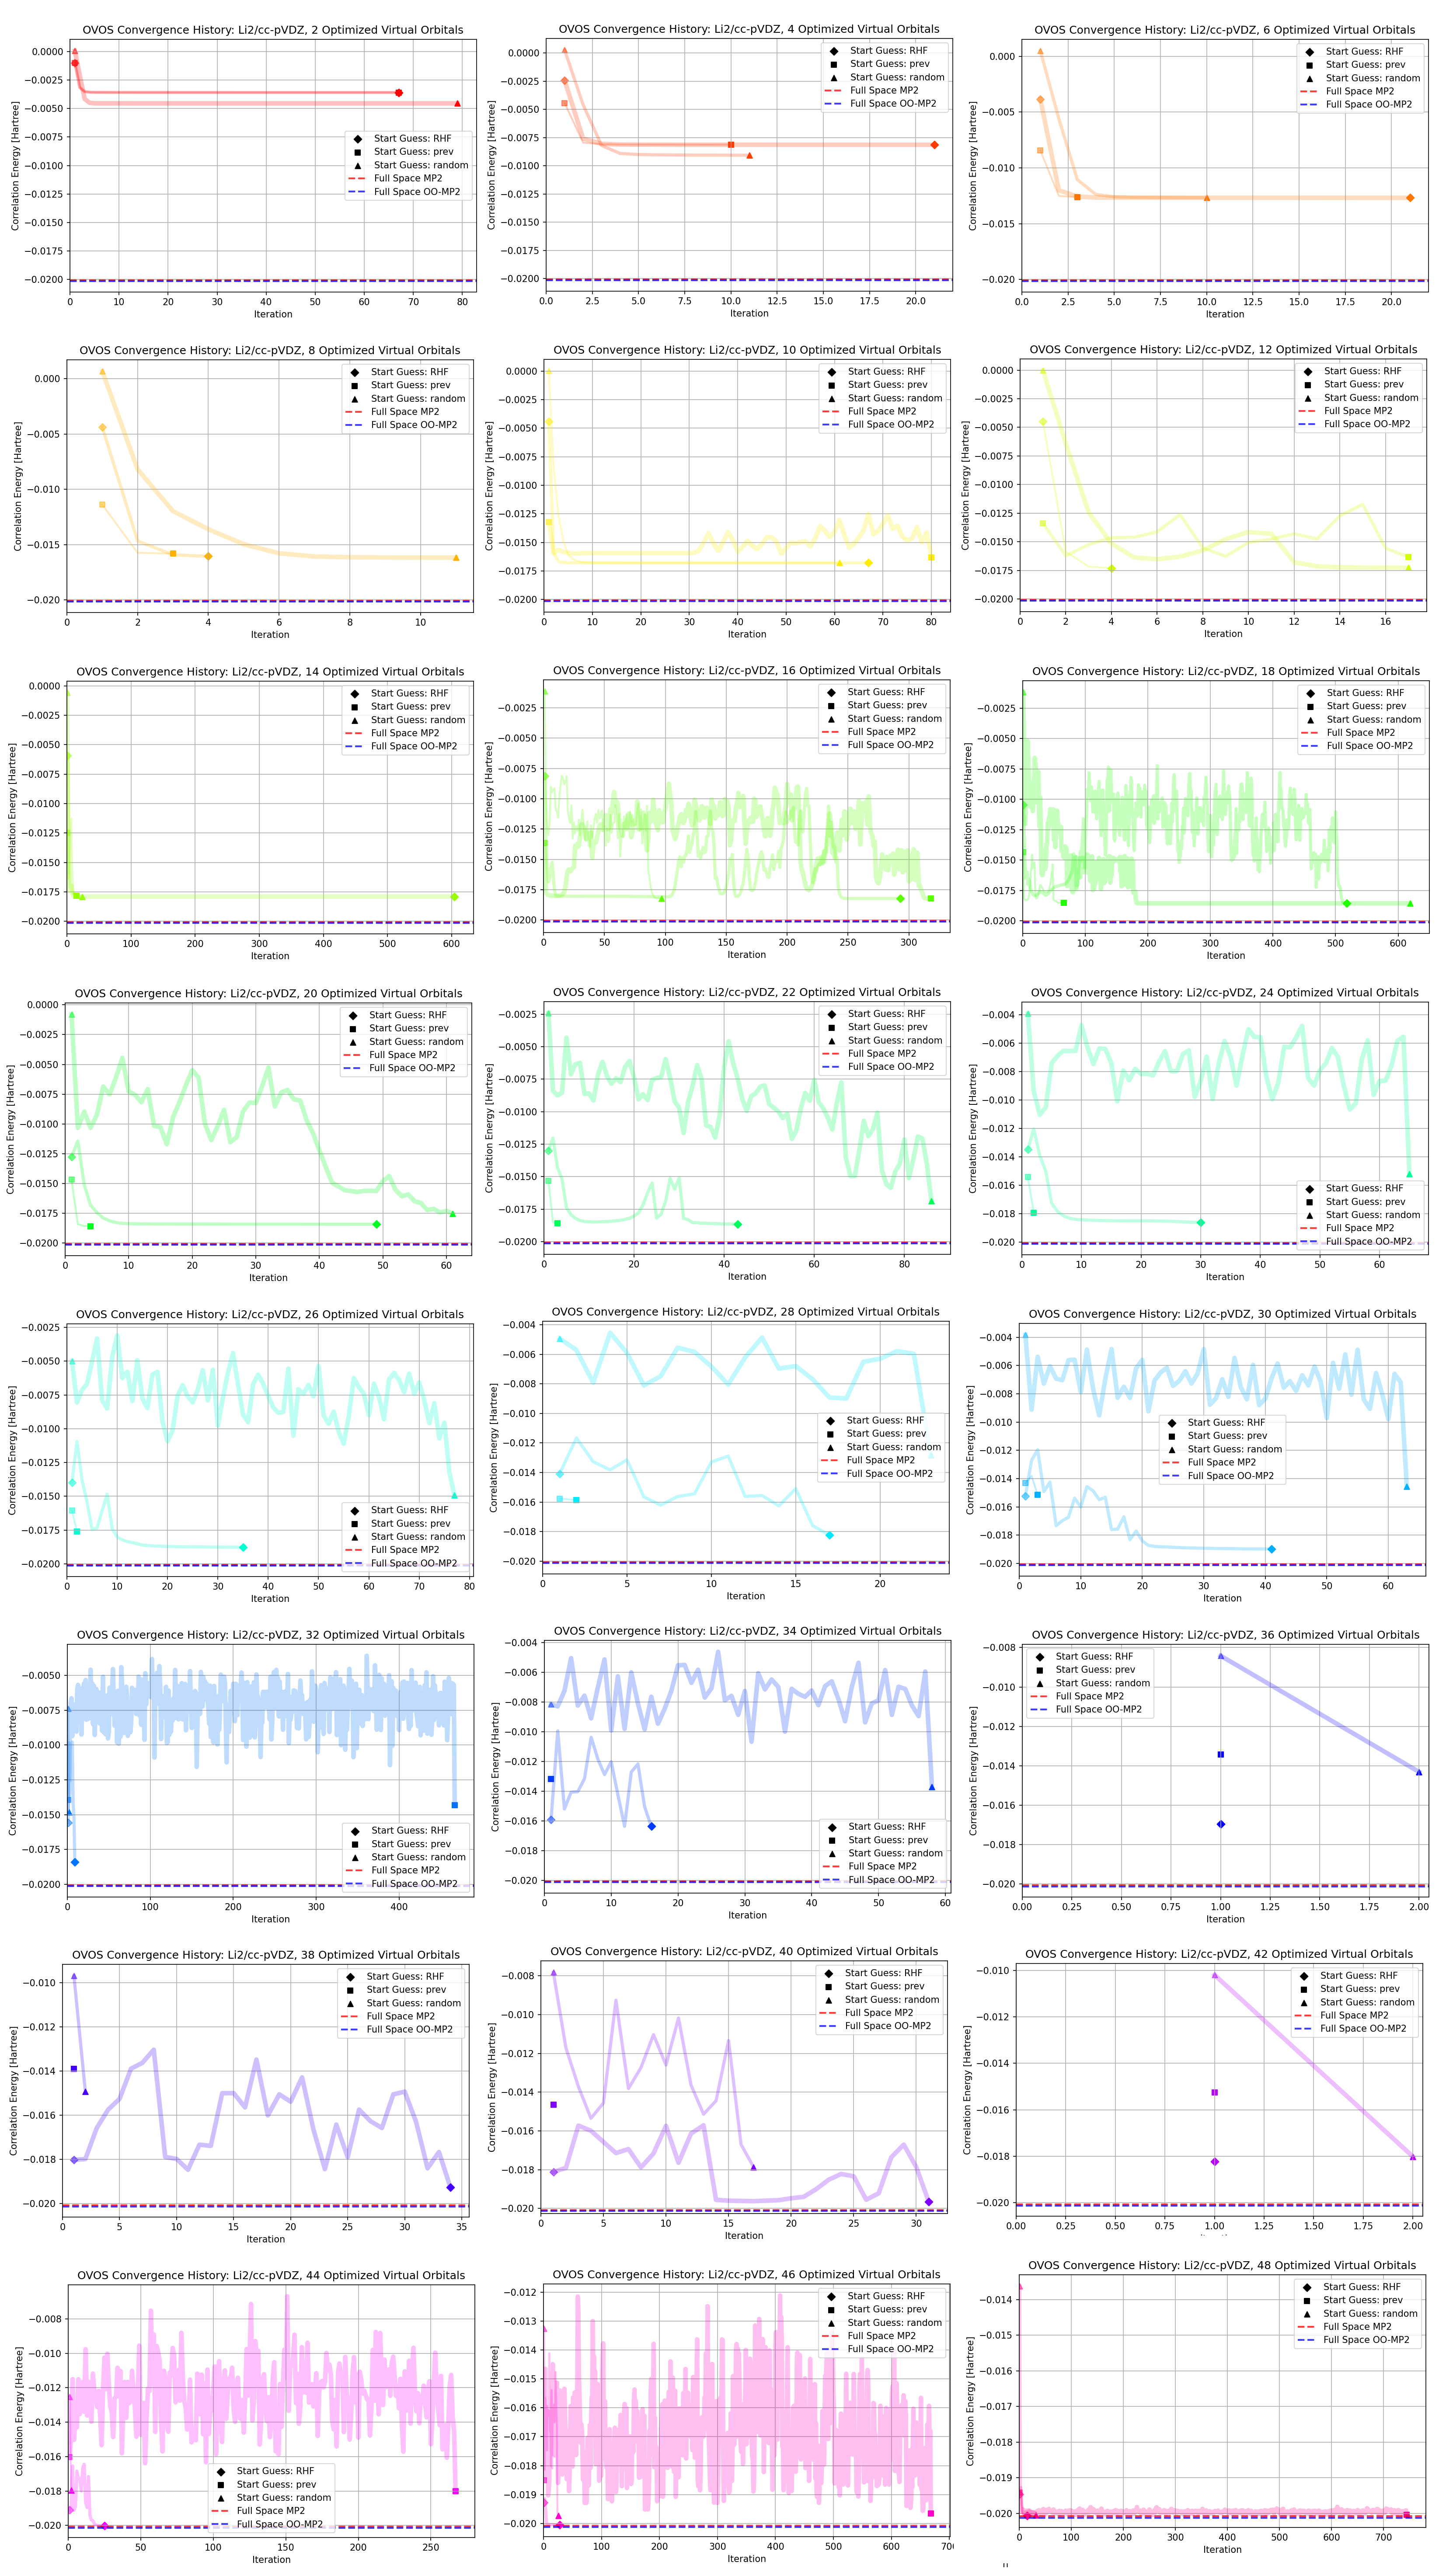
\includegraphics[width=0.7\textwidth]{figures/Ekstra/OVOS_conv_Li2_cc-pVDZ.png}
    \caption{Li$_2$/cc--pVDZ OVOS convergence history for each active unoccupied orbitals, colour coded to fit the OVOS convergence plot in Figure~\ref{fig:appb_MP2_6-31G_ovos} and in Section~\ref{subsec:results_ovos_mp2}. The OVOS algorithm takes RHF (diamond), previous (square), and random (triangle) as start guesses. Dashed lines: full-space MP2 (red), OO-MP2 (blue), FCI (green) references.}
    \label{fig:appb_conv_Li2_cc-pVDZ_ovos}
\end{figure}

\newpage

\begin{figure}[H]
    \centering
    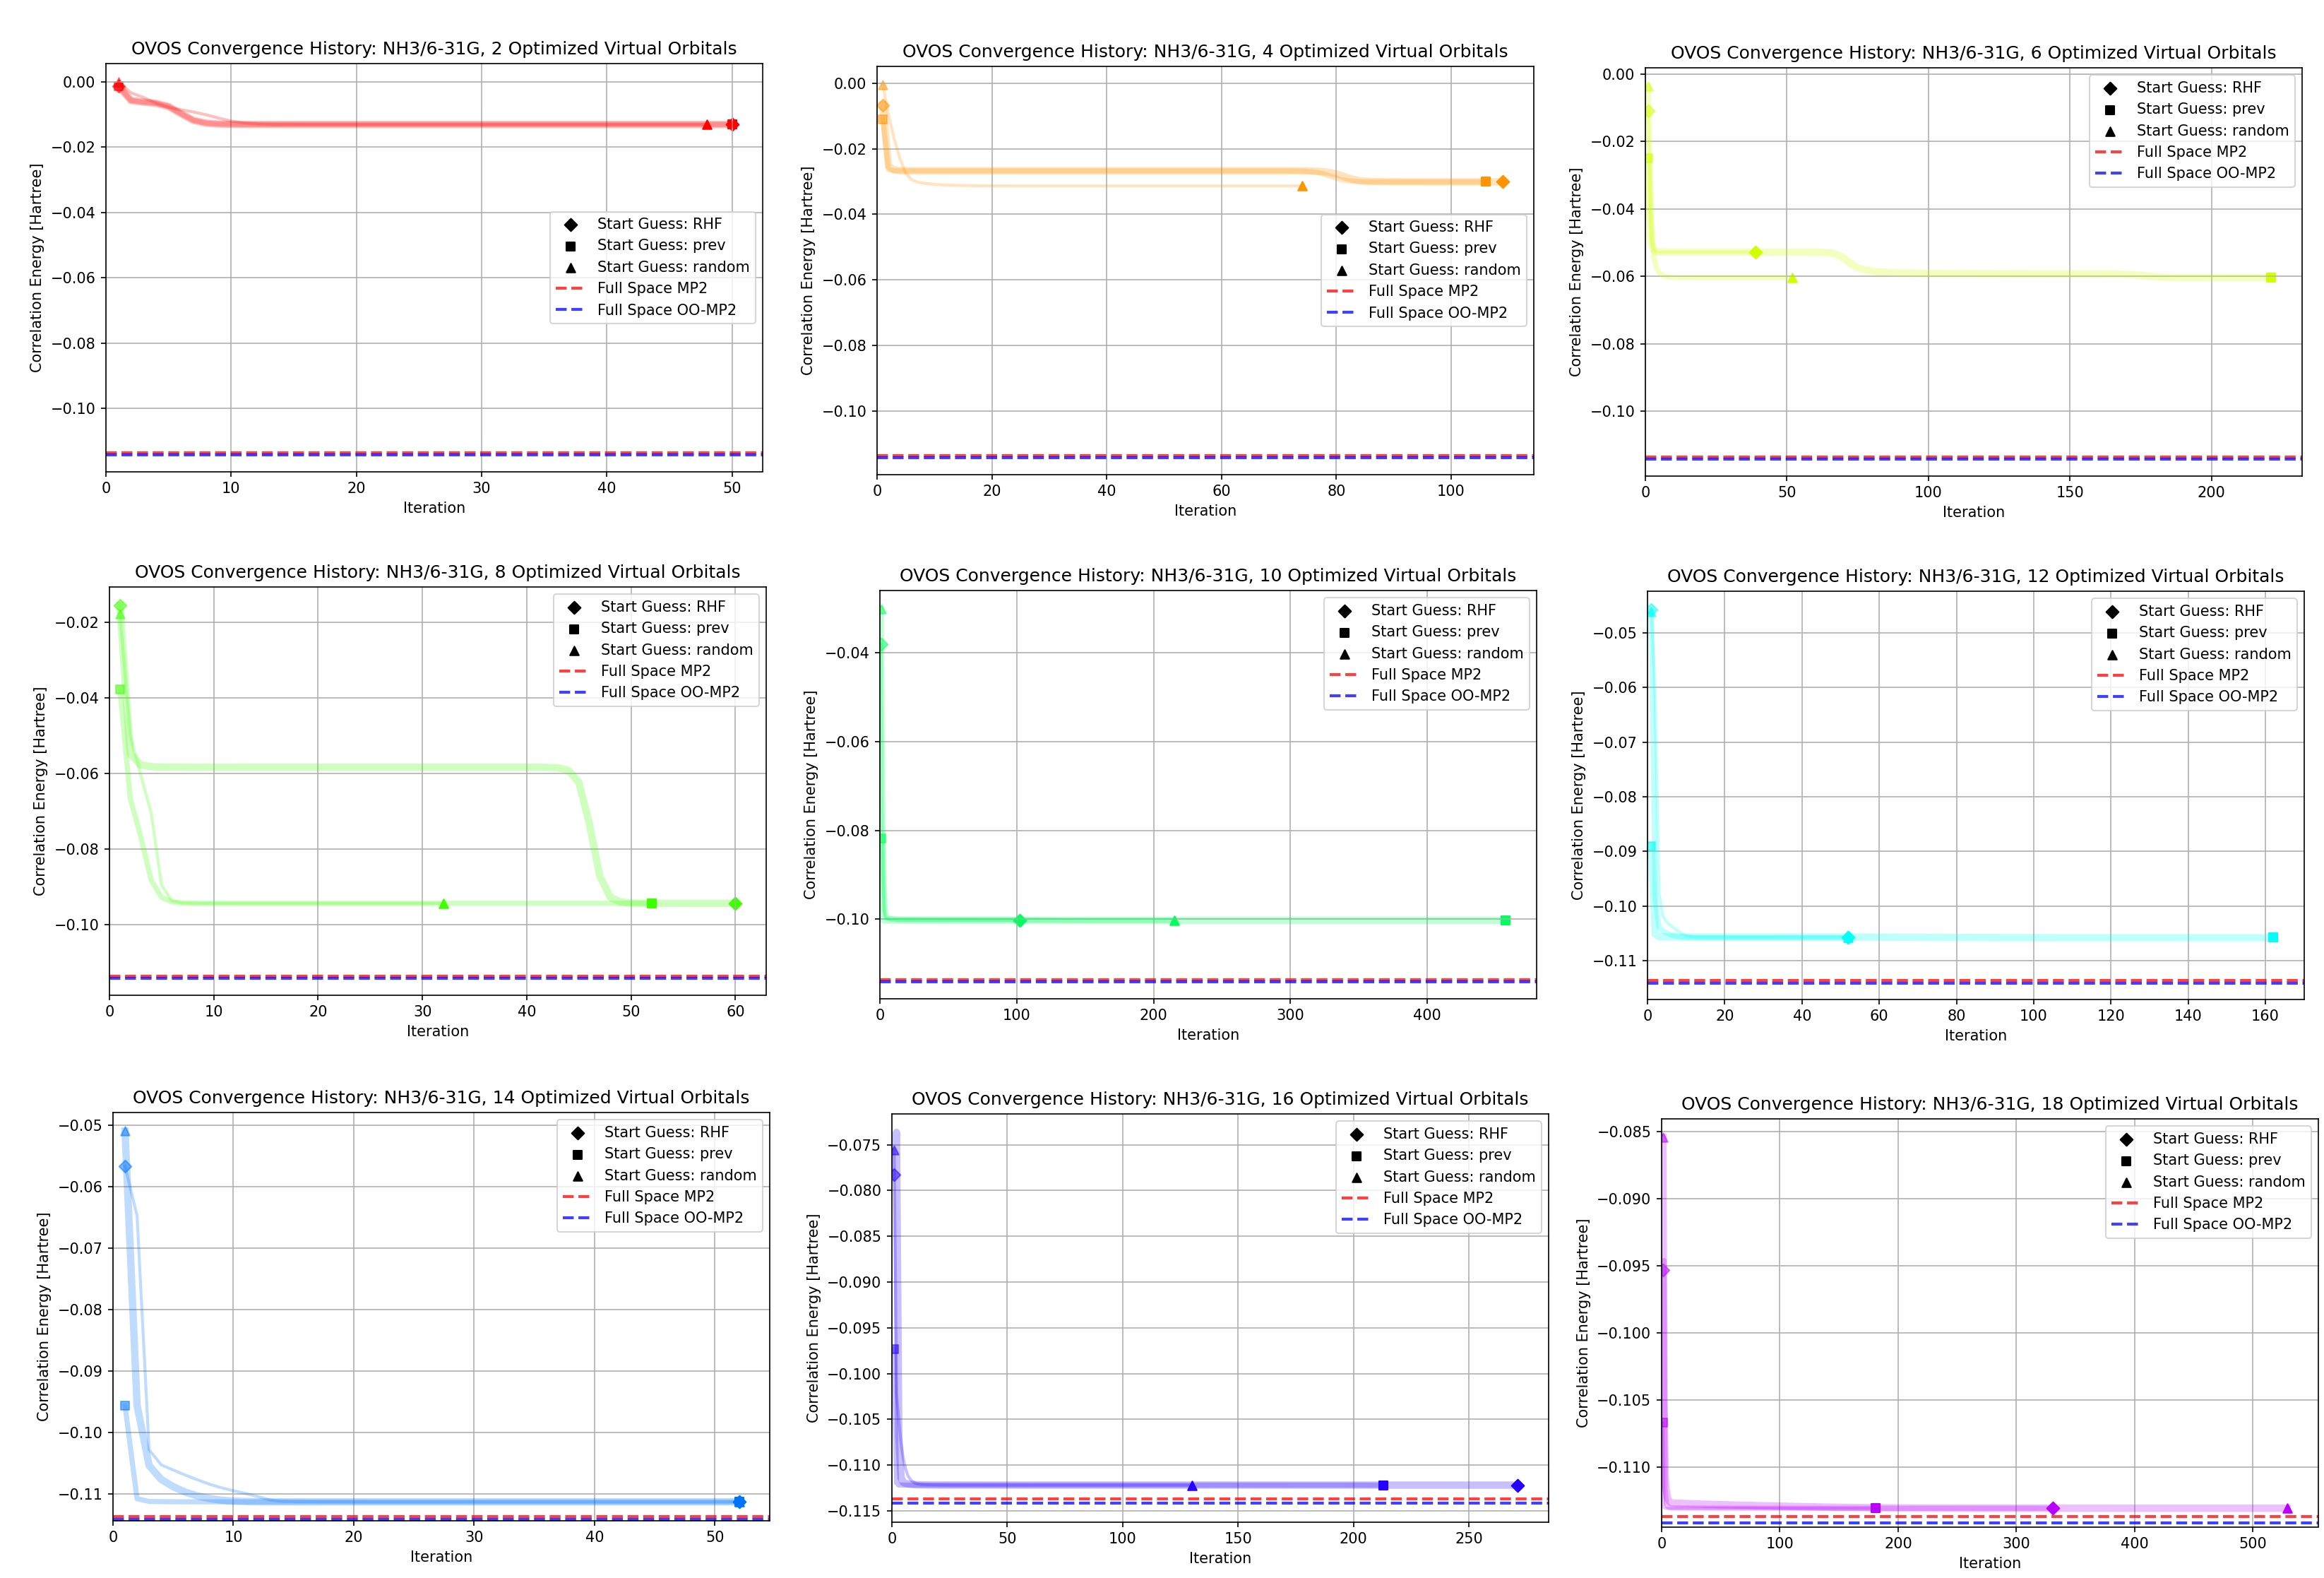
\includegraphics[width=0.9\textwidth]{figures/Ekstra/OVOS_conv_NH3_6-31G.png}
    \caption{NH$_3$/6--31G OVOS convergence history for each active unoccupied orbitals, colour coded to fit the OVOS convergence plot in Figure~\ref{fig:appb_MP2_6-31G_ovos} and in Section~\ref{subsec:results_ovos_mp2}. The OVOS algorithm takes RHF (diamond), previous (square), and random (triangle) as start guesses. Dashed lines: full-space MP2 (red), OO-MP2 (blue), FCI (green) references.}
    \label{fig:appb_conv_NH3_6-31G_ovos}
\end{figure}

\newpage

\begin{figure}[H]
    \centering
    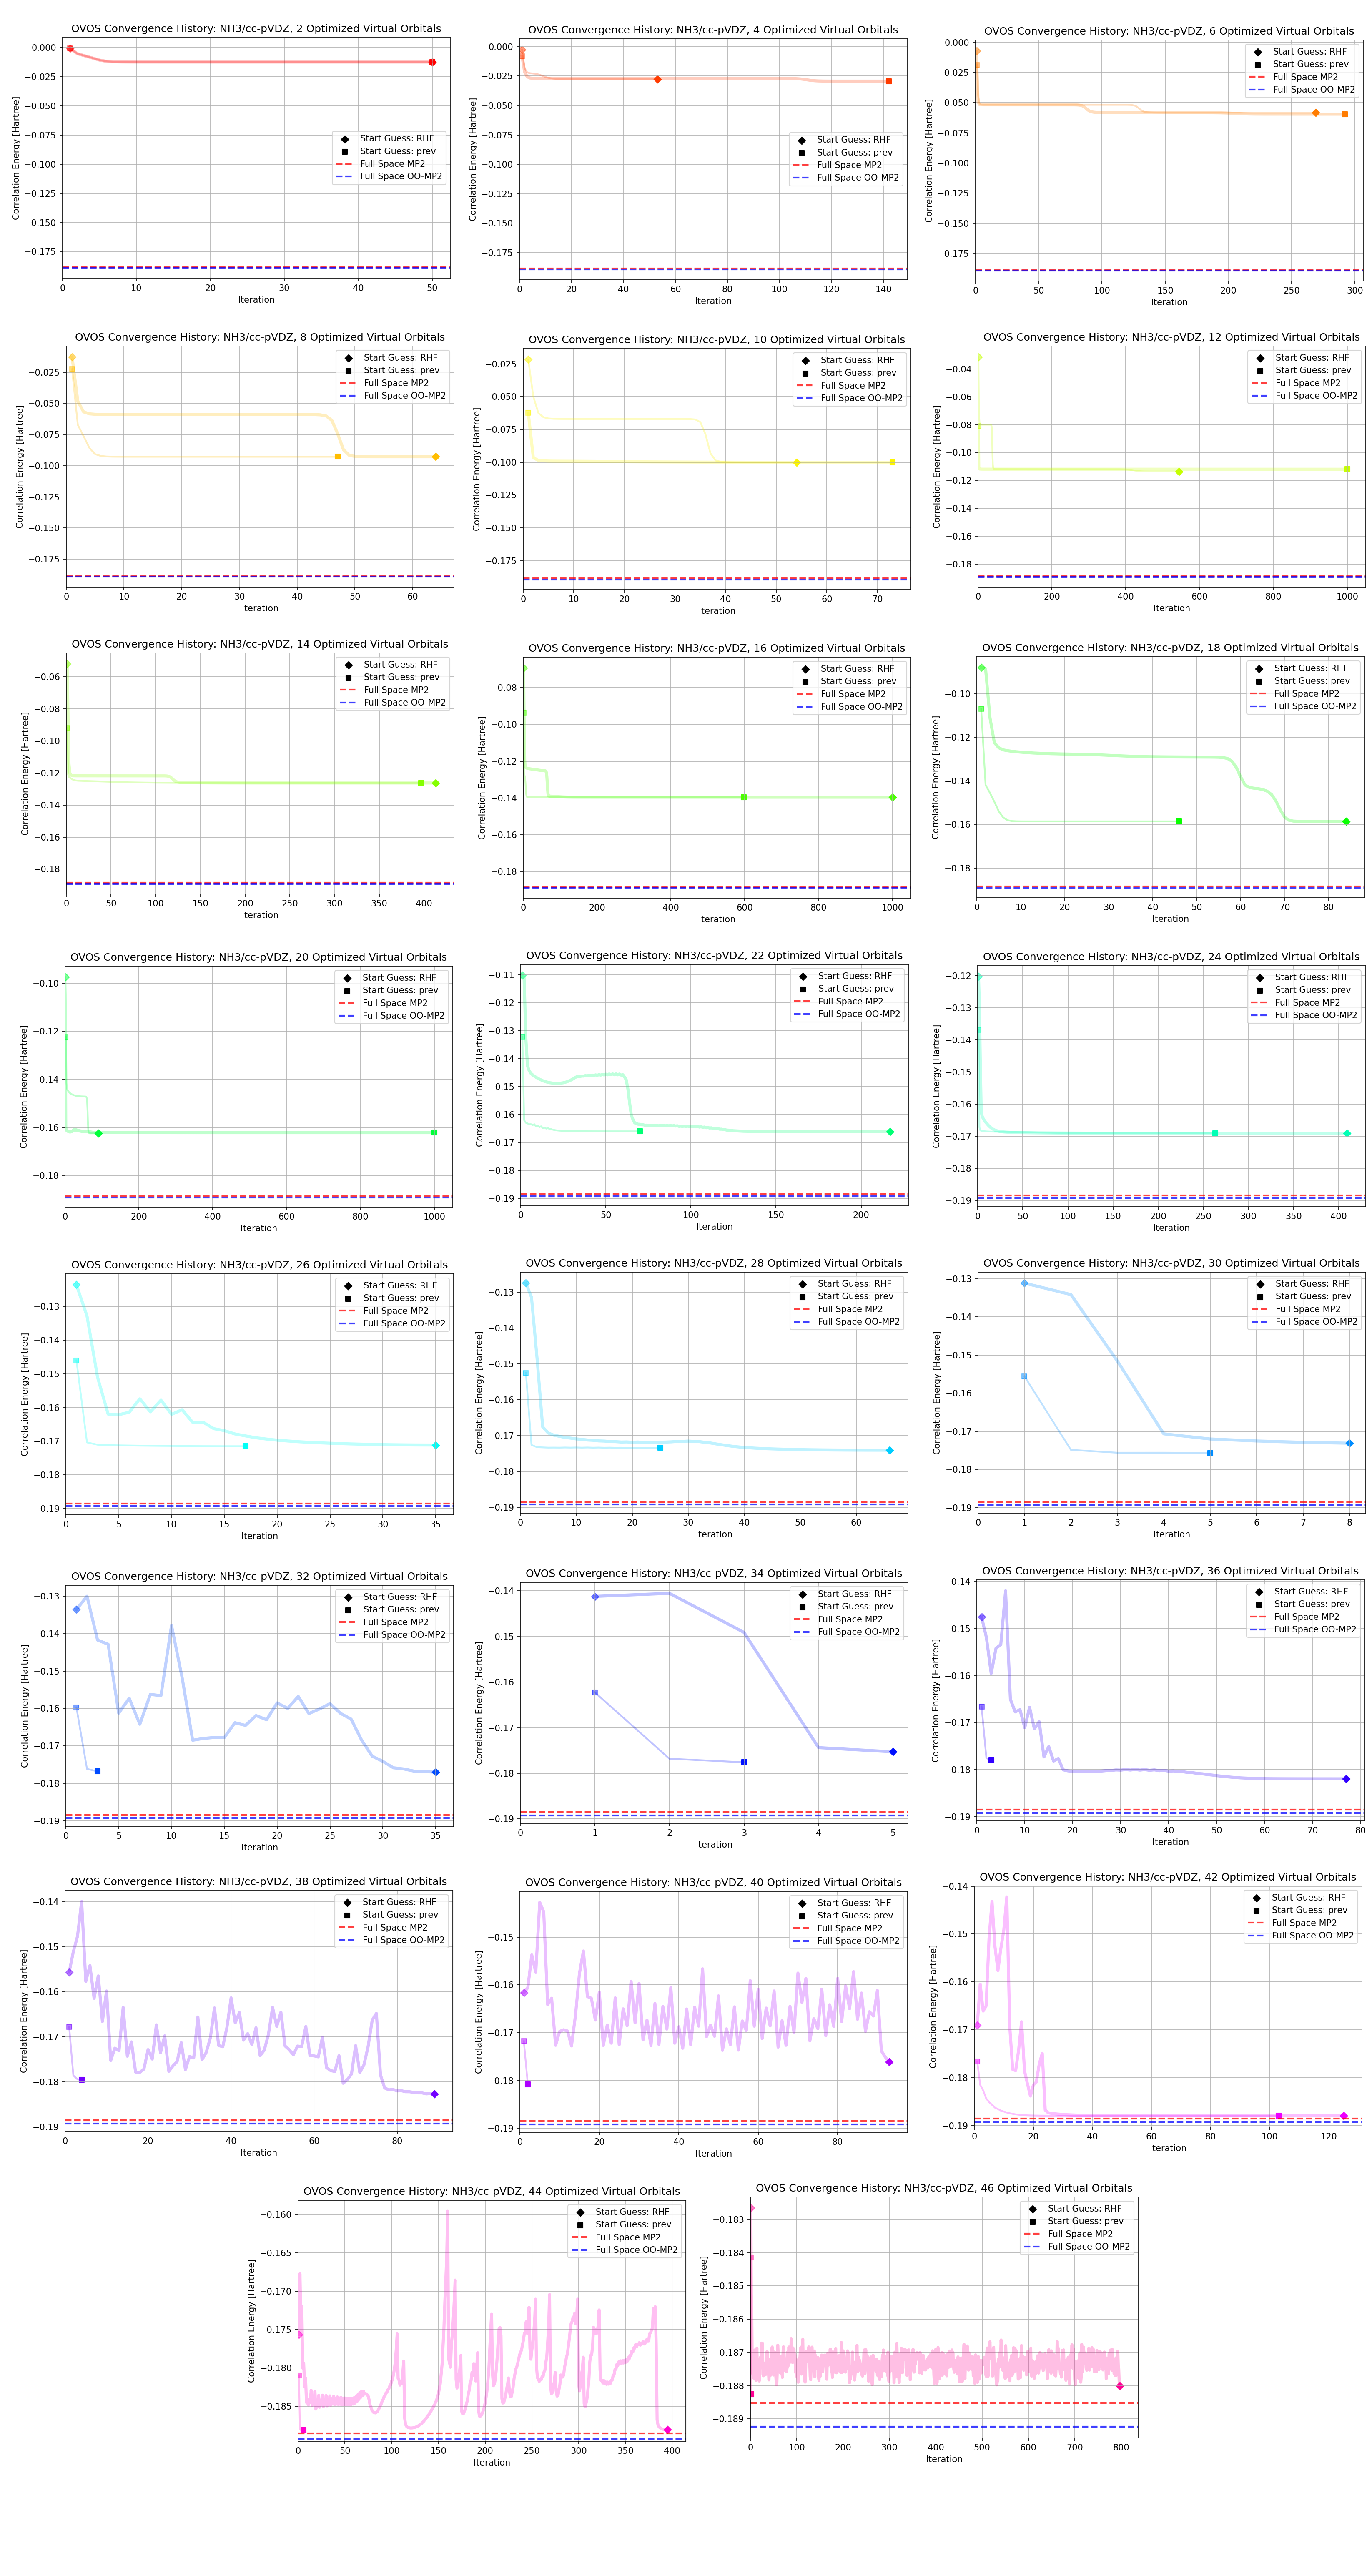
\includegraphics[width=0.8\textwidth]{figures/Ekstra/OVOS_conv_NH3_cc-pVDZ.png}
    \caption{NH$_3$/cc--pVDZ OVOS convergence history for each active unoccupied orbitals, colour coded to fit the OVOS convergence plot in Figure~\ref{fig:appb_MP2_6-31G_ovos} and in Section~\ref{subsec:results_ovos_mp2}. The OVOS algorithm takes RHF (diamond), previous (square), and random (triangle) as start guesses. Dashed lines: full-space MP2 (red), OO-MP2 (blue), FCI (green) references.}
    \label{fig:appb_conv_NH3_cc-pVDZ_ovos}
\end{figure}

\newpage

\section{OVOS Figures}

Here we include illustrative figures of the OVOS loop structure, which provide a visual representation of the algorithm's workflow.

\begin{figure}[H]
    \centering
    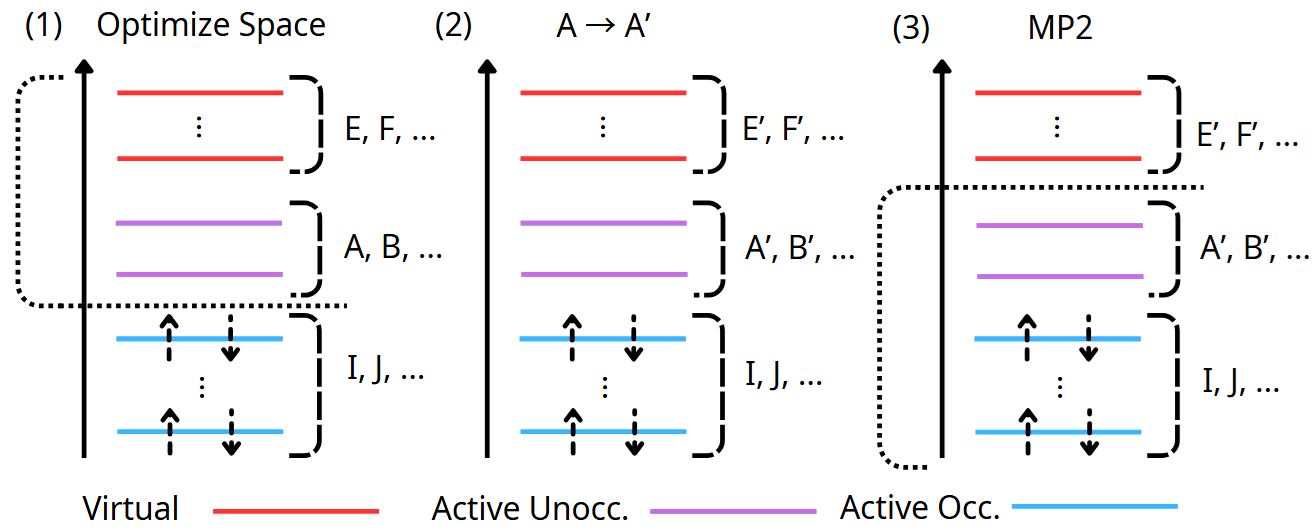
\includegraphics[width=0.9\textwidth]{figures/Ekstra/OVOS_loop.png}
    \caption{Illustration of the OVOS loop structure, showing the flow of the algorithm's loop, the optimization of virtual orbitals.}
    \label{fig:appb_ovos_loop_structure}
\end{figure}




